%%% Clinic Statement of Work Template
%%%
%%% C.M. Connelly <cmc@math.hmc.edu>
%%%
%%%  $Id: statement-of-work-template.tex 353 2010-08-23 23:47:44Z cmc $


%%% !!! HMC STUDENTS SHOULD REMOVE THE FOLLOWING COPYRIGHT NOTICE FROM
%%% !!! FINAL SUBMISSIONS.

%%% Copyright (C) 2004-2010 Department of Mathematics, Harvey Mudd College.
%%%
%%% This file is part of the hmcclinic class document provided to
%%% HMC mathematics students.
%%%
%%% See the COPYING document, which should accompany this
%%% distribution, for information about distribution and
%%% modification of the document and its components.

%%% !!! END COPYRIGHT NOTICE.


%%% Clinic reports use the clinic class, which should be located
%%% somewhere in TeX's search path.

%%% For your ``statement of work'' (or ``work statement''), specify
%%% the ``proposal'' document-class option to the hmcclinic class.
\documentclass{hmcclinic}
\usepackage{graphicx}
\usepackage{enumerate}
\usepackage{paralist}

%%% The major difference between the statement of work and a midyear
%%% or final report is that the statement of work is typeset as an
%%% article, which means that the highest level of structural
%%% division available to you is section rather than chapter.

%%% There are also some changes in pagination styles and content
%%% that reflect the briefer nature of the proposal.  For example,
%%% in the longer reports, you use \frontmatter, \mainmatter, and
%%% \backmatter to separate some sections of the report from
%%% others.  In the statement of work, you don't need those
%%% commands, as no such division is necessary.

%%% Other packages needed by your document may be loaded here.
% \usepackage{url}              % For formatting URLs and other web or
                                % file references.

%%% Provide additional context around errors. 
\setcounter{errorcontextlines}{1000}


%%% Information about this document.

%%% I find it most useful to put identifying information about a
%%% document near the top of the preamble.  Technically, this
%%% information must precede the \maketitle command, which often
%%% appears immediately after the beginning of the document 
%%% environment.  Placing it near the top of the document makes it
%%% easier to identify the document, and keeps it out from getting
%%% mixed up with the real meat of the document.

%%% We use the same set of commands for specifying information about
%%% the people involved with the project that are used in the longer
%%% reports, so you can copy most of this information directly into
%%% your midyear and final reports.

%%% So, some questions.

%% What is the name of the company or organization sponsoring your project?
\sponsor{SpaceX}

%% What is the title of your report?
\title{Process Time Analysis In Spaceflight}

%% Who are the authors of the report (your team members)?  (Separate
%% names with \and.)
\author{Wendy Brooks~(Fall Project Manager) \and May Lynn Forssen~(Spring Project Manager) \and Alix Joe \and
Rachel Macfarlane}

%% What is your faculty advisor's name?  (Again, separate names with
%% \and, if necessary.)
\advisor{Ben Wiedermann}

%% Liaison's name or names?
\liaison{Jim Gruen \and Jessica Hester '13 \and Jesse Keller }

%%% End of information section.

%%% New commands and environments.

%%% You can define your own commands and environments here.  If you
%%% have a lot of material here, you might want to consider splitting
%%% the commands and environments into a separate ``style'' file that
%%% you load with \usepackage.

\newcommand{\coolcommand}[1]{#1 is cool.} % Lets everyone know that
                                % the person or thing that you provide
                                % as the argument to the command is
                                % cool.

\newcommand{\tracecmd}{\fontfamily{pcr}\selectfont trace-cmd}

%%% Some theorem-like command definitions.

%%% The \newtheorem command comes from the amsthm package.  That
%%% package is loaded by the class file.

%%% Note that these definitions have changed from the version in the
%%% sample report document by dropping the ``within'' argument.  See
%%% Gratzer's _Math into LaTeX_ or the AMS-LaTeX documentation for
%%% more details.

% \newtheorem{thm}{Theorem}
% \newtheorem{Theo1}{Theorem}
% \newtheorem{Theo2}{Theorem}
% \newtheorem{Lemma}{Lemma}


%%% If you find that some words in your document are being hyphenated
%%% incorrectly, you can specify the correct hyphenation using the
%%% \hyphenation command.  Note that words are separated by
%%% whitespace, as shown below.

\hyphenation{ap-pen-dix wer-ther-i-an}


%%% The start of the document!

%% The document environment is the main environment in any LaTeX
%% document.  It contains other environments, as well as your text.

\usepackage{float}
\restylefloat{table}
\begin{document}

%%% In a longer document (such as your midterm and final reports),
%%% you would have separate \frontmatter, \mainmatter, and
%%% \backmatter commands to define some large chunks of your
%%% document.  For the Statement of Work, which is a short document,
%%% we don't need these commands.

%%% Your Statement of Work begins with a title page.  The title page
%%% is formatted by commands in the document class file, so you
%%% don't need to worry about what it looks like -- just putting the
%%% \maketitle command in your document (and filling in the necessary
%%% information for the identification commands above) is enough.
\maketitle
 
\tableofcontents
%%% In a longer document or an article being submitted to a journal
%%% or conference, you would probably have an abstract that
%%% summarized the purpose of the document.  We don't need that for
%%% a Statement of Work.

%%% Similarly, in longer documents you would probably have commands
%%% to include a table of contents and lists of figures or tables.
%%% For a short document such as the Statement of Work, we don't
%%% need these commands.


%%% Content.
\chapter{Background and Project Goals} % May Lynn
%\section{Introduction}

SpaceX is an American space transport company that designs and manufactures
advanced rockets and spacecraft. SpaceX rockets depend on a variety of software
to be successful, including simulations, flight software, and data analysis.
Almost all of this software is written in-house and is complex enough that subtle
problems are often hard to catch and very time consuming to debug.

%\section{Background} % May Lynn
%\section{Tracing and Debugging}

The data that SpaceX developers use to find software bugs is called
a {\bf kernel trace}, which documents the different tasks running on a computer over a
certain span of time, keeping track of when each task was running on each processor. 

% Several computers are on board each SpaceX rocket and rely on tasks running in
% predictable, cyclical patterns to coordinate. An unexpected preemption, priority
% inversion, or some break in the pattern of tasks being run can cause problems
% for the rocket.
To find potential bugs in their software, SpaceX developers look for
problems like unexpected preemptions, priority inversions, and breaks in the
pattern of tasks being run.
 A {\bf preemption} occurs when one program is running, and
is then blocked by another program starting to run on the same CPU. 
A {\bf priority
inversion} occurs when a high-priority task is indirectly blocked by something of
lower priority using a shared resource that the higher priority task needs in
order to run. 

The software running on SpaceX rockets has deadlines for tasks at regular intervals because timing is very important in rocket flight. When there is a break in this cyclical pattern of processes this means that there is likely a bug in the software. These cyclical patterns of processes are called ``cycles''.

%\section{Existing Tool}
SpaceX currently uses a tool called KernelShark %%TODO FIXME citation
to visualize trace data and help find any bugs or anomalies (Figure 1.1). 
SpaceX engineers look for anomalies in process timing, which often indicates 
software problems on the rocket. We were informed by our liaisons that this
 debugging process can take up to several days, 
which is an inefficient use of engineer's time. \\

\begin{figure}[H]
  \centering
      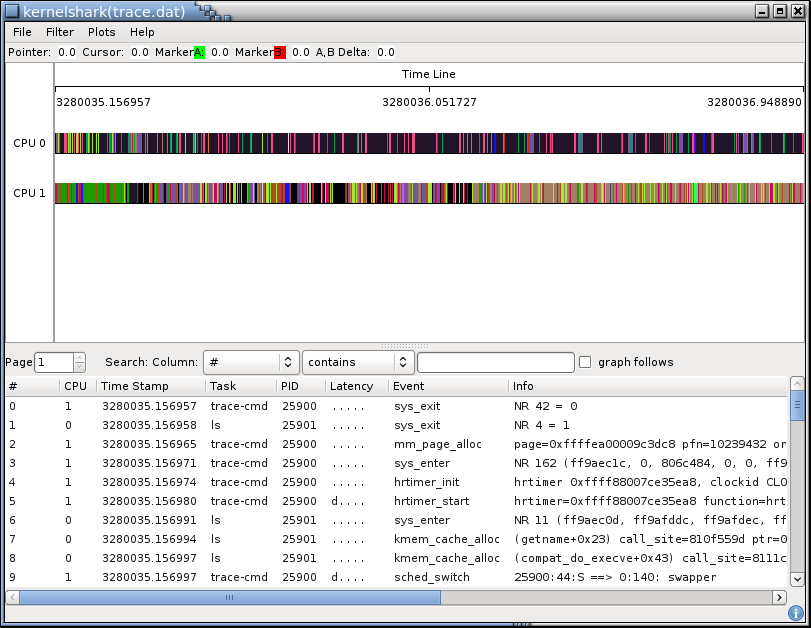
\includegraphics[width=4.95in]{kshark-open.png}
  \caption{KernelShark consists of a graphical display of the programs running on a computer over time (top half of screen), as well as a tabular view of the same information, in the form of CPU events such as processes switching, waking, or sleeping (bottom half of screen).}
\end{figure}

KernelShark displays the data but provides limited ways to interact with it. It
does not have many features geared towards finding anomalies and has no tools for
dealing with cycles.  In order to utilize information about cycles, the user
must recognize by sight alone where cycles start and end, which is very
difficult. Users are only able to compare cycles by moving back and forth on
the timeline KernelShark provides, also a time consuming process.

KernelShark has a poorly designed UI that does not function as expected. The
events table at the bottom of KernelShark is not searchable, nor can the columns
be sorted. When a user wants to display a specific task, they must choose from
an unsortable and unsearchable list of tasks that might be hundreds of tasks
long. Additionally, zooming out on KernelShark's visual timeline is
uninituitive and confusing.

%Using only this visualization, it can be difficult to see where the cyclical
%deadlines for the programs begin and end, making it hard to find when something
%misses a deadline. In addition, the tabular display of the CPU events in the
%bottom part of the screen has minimal search functionality and the different
%columns of the table are not sortable. Individual timelines for tasks can be
%displayed below this main chart, but the menu to select a task does not have
%any searching capability and does not order the tasks in any discernible way.

%\section{Project Goals} % May Lynn
The goal of this project was to make it easier and faster for SpaceX engineers
to find software problems by creating a tool that visualizes rocket data and
highlights problem areas. We have created an improved user experience and
provided more visualizations of the data than the old tool. 
\chapter{SpaceShark}

\section{Obtaining SpaceShark}
  Our code is publicly available on GitHub at
\begin{center}
  github.com/golden3point14/SpaceX14
\end{center}
The README of this repository provides a link to download a
  64 bit Linux version of the application. This release is a zip file that
  contains an executable, the parser, a short wrapper script, and two additional
  files that are necessary to get the executable to run: \texttt{nw.pak} and
  \texttt{icudlt.dat}.
  The short wrapper script is called \texttt{spaceshark} and has the following usage:

\begin{verbatim}spaceshark [-p | --parse filename] [-o | --open filename] 
           [ -h | --help]\end{verbatim}

  The first option allows the user to pass an unparsed trace file to the
  application. The parser will be run and pass its output 
  to the application as it opens, skipping the load page that asks the
  user to choose a file. The second option allows the user to pass a
  JSON file, the output format our parser uses, to the application. Finally, using the \texttt{-h} flag or any option
  not recognized by the script will display the usage and a description of
  available options.

\section{Design}

  SpaceShark helps SpaceX engineers find scheduling related problems.
  SpaceShark is composed of pages that each give a different view of the data,
  from a complete overview down to the details of of a single task. A brief
  summary of each page and its intended purpose is given below.

  \begin{center}
    \begin{tabular}{p{0.2\linewidth}p{0.7\linewidth}}
     \toprule
      Page Name       & Purpose\\
      \midrule
      Load File       & Allow a user to choose the data to import into the
      application\\
      Overview        & Provide user overall view of the data\\
      Cycles          & Break data into intervals so that a user can compare
      across them\\
      Task Statistics & Give user high-level statistics about the data,
      comparing task's total runtimes and preemptions\\
      Task State      & Display a single tasks actions and interactions\\
      Task Compare    & Allow a user to compare several tasks changes in state
      over time\\
    \bottomrule
    \end{tabular}
  \end{center}
\subsection{Example User Flow}
  The SpaceX debugging process involves several steps.  A user will navigate
  through the tool differently depending on what level of information they
  already have.

  If a user suspects that a particular task is involved in the problem, they
  could immediately navigate to the Task State page. From this, they are able to
  see if the task was unexpectedly preempted. These tasks are displayed in the
  table of preemptions, or when hovering over a preemption event in the graph
  below it.

  If a user does not have any suspicions about what happened, they could instead
  navigate to the Cycles page. By comparing the patterns of tasks run during
  different cycles, it should be easy to see an abnormal sequence of tasks. The
  user can then hover over this sequence on the chart and read which tasks are
  running. A user might also navigate to the Task Statistics page to quickly see
  if any task is preempted far more than expected. This task could then be
  viewed on the Task State page, as described above.

%  There are many other possible ways users might navigate through the
%  application, but the team believes the Cycles page and Task State page 
%  are especially useful.
%
%  Each page is described in more detail in the following sections.

\subsection{Load File Page}

\begin{figure}[H]
  \centering
      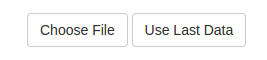
\includegraphics[scale=0.75]{loadFile-buttons.png}
  \caption{Choose File selects a new file and Use Last Data selects the file
  that was most recently loaded into the tool. The Use Last Data option will not
display if no data has ever been loaded.}
  \end{figure}

\paragraph{Purpose:}
When the user opens SpaceShark, they see the Load File page (Figure 2.1).  This
page allows the user to choose which data to load, or to choose to load the data
that was most recently used.  The user can easily resume their work by choosing
the second option, as both the data and the state of each page during the user's
previous session are reloaded.

\paragraph{Interactivity:}
The user can click either the ``Choose File'' button to choose a new file to view, or if they have viewed a file using our tool before, they can click the ``Use Last Data'' button to see the data that they were previously viewing.

\paragraph{Comparison to KernelShark:}
KernelShark does not allow the user to easily resume viewing previous data. SpaceX engineers often want to be able to save and revisit their work at a later time. 

%The code for the Load File page can be found in assets/js/loadFile.js.

  \subsection{Overview Page} 
  
  \begin{figure}[H]
  \centering
      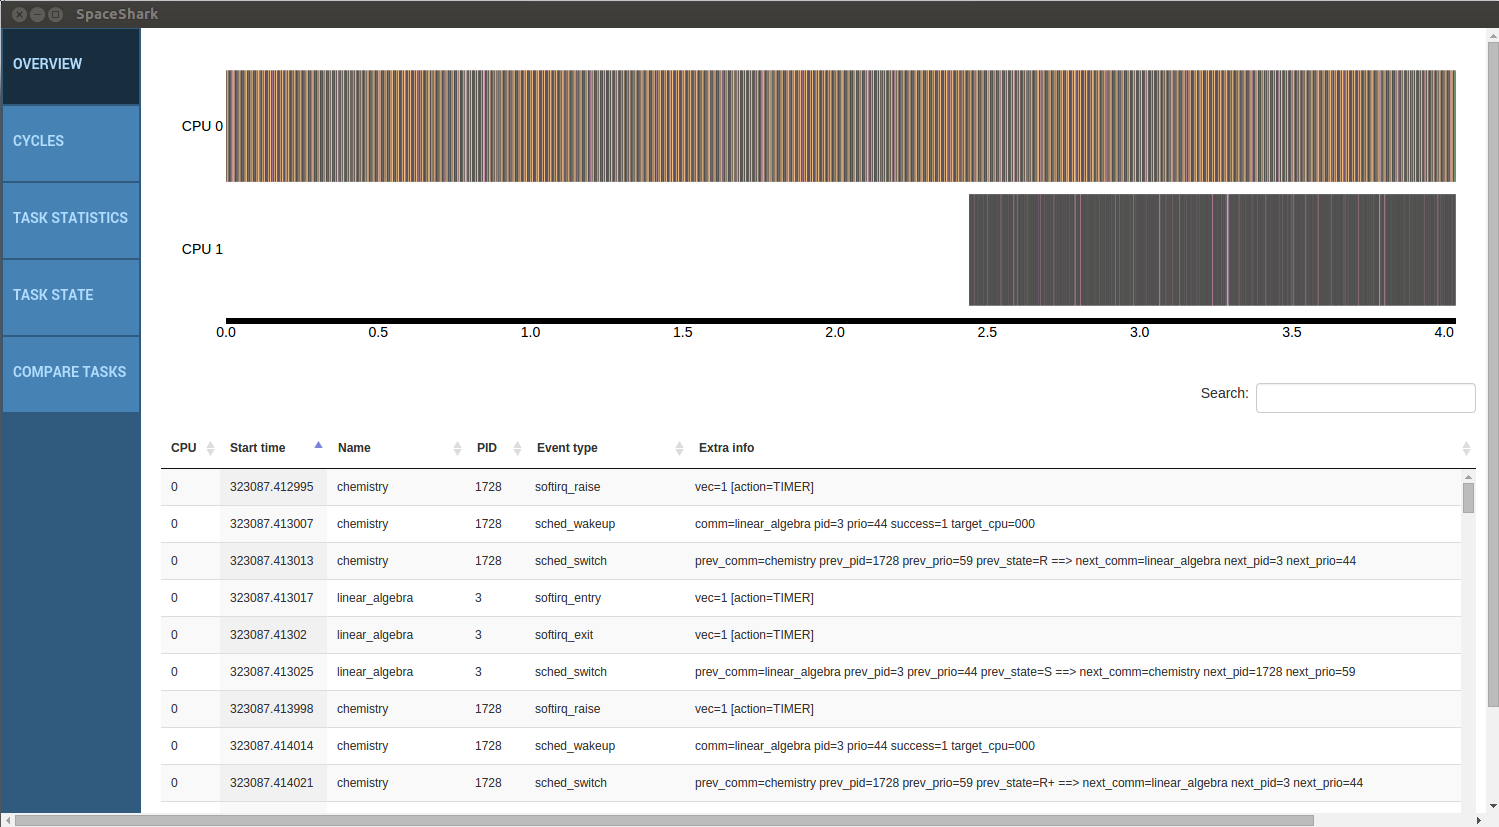
\includegraphics[width=5in]{overview-page.png}
  \caption{The top chart shows a graphical display of the programs running on the computer over time, and the bottom table shows a tabular version of this same information.}
  \end{figure}

\paragraph{Purpose:} 
The goal of the Overview page is to give a broad view of the data, displaying
all of the data at once.  The users sees a chart of the programs that were
running on each of the CPUs for the entire duration of the trace and a table
listing all of the events in the trace.

\paragraph{Interactivity:} The user can zoom in and out on the graph by using
the mouse scroll wheel, and pan left and right by clicking and dragging.
Double-clicking on the graph also zooms in on it. The user can hover over any
event on the graph to see a text box with more information about that particular
event.  This information consists of the task name, the CPU it's running on, its
process ID (PID), duration, and information about the task it displaced from the
CPU, including this task's name, priority, and resulting state (runnable or
sleeping). Clicking on an event displayed in the graph will cause the
events list to scroll to that event.

The columns of the table consist of the CPU, start time, name, PID, event type,
and extra information dependent on the event type. By default, the table is
displayed in ascending order of time.  Hovering over any of the table cells
highlights that entire row. Users can also double click on an event to be
redirected to that task on the Task State page.  The search feature filters out
entries that do not match the search text in any column.  Clicking on any of the
column headers orders the information in the table by the contents of that
column.  Below the table, the user can see the total number of entries and the
range of entries currently on the screen.

\paragraph{Comparison to KernelShark:} 
  KernelShark's main interface looks very similar to the Overview page, but
  sometimes failed to correctly filter and search for events. With this page,
  we retained important functionality from the old tool. We expand on the
  functionality of the old tool in other pages.

  KernelShark also has graph plots of the CPUs and includes similar features. A
  user can zoom by clicking and dragging a rectangular box, from left to right,
  over the graph.  This allows the user to precisely view a specific area of the
  graph.  Although this zoom functionality seems helpful, it doesn't follow
  common zoom functionalities of a modern day desktop application. Zooming out of
  the graph in KernelShark is also unintuitive: the user can click and drag a
  rectangular box, from right to left, over the graph. This technique
  does not give the user any kind of information about how much the graph is
  zooming out and can therefore be confusing to users. When
  zooming on KernelShark, a horizontal bar appears at the bottom of the graph to
  be able to easily pan.
    
  KernelShark has the same functionality as our tool of being able to click on a
  spot in the graph and have the table scroll to that event. 
    
  The feature of hovering over the graph to get more information also exists in
  KernelShark, and the team and liaisons felt that it would be useful to have in
  SpaceShark.

  Like our tool, KernelShark has a list of events on the bottom half of their
  tool and gives users the option to search and filter events in the
  table view.

  In KernelShark, the user can select individual tasks to plot on the same graph
  as the CPUs. To maximize space on the Overview page, we decided to move this
  feature to its own page.

  KernelShark users can opt to display certain CPUs instead of all of them at
  once. We felt that this feature was not necessary because SpaceX trace files
  generally have few CPUs, which is not a problem in terms of page space on the
  Overview page.


%    The code for the Overview page is found within assets/js/main.js. This file is
%    responsible for fetching and loading the data, creating a timeline
%    visualization that the user can pan and zoom into, and creating a table that
%    lists all events in the trace. The code for the chart and table is found in
%    gantt-chart-d3.js and dataTables.scroller.js, respectively.
    
  \subsection{Cycles Page} %Alix

  \begin{figure}[H]
  \centering
      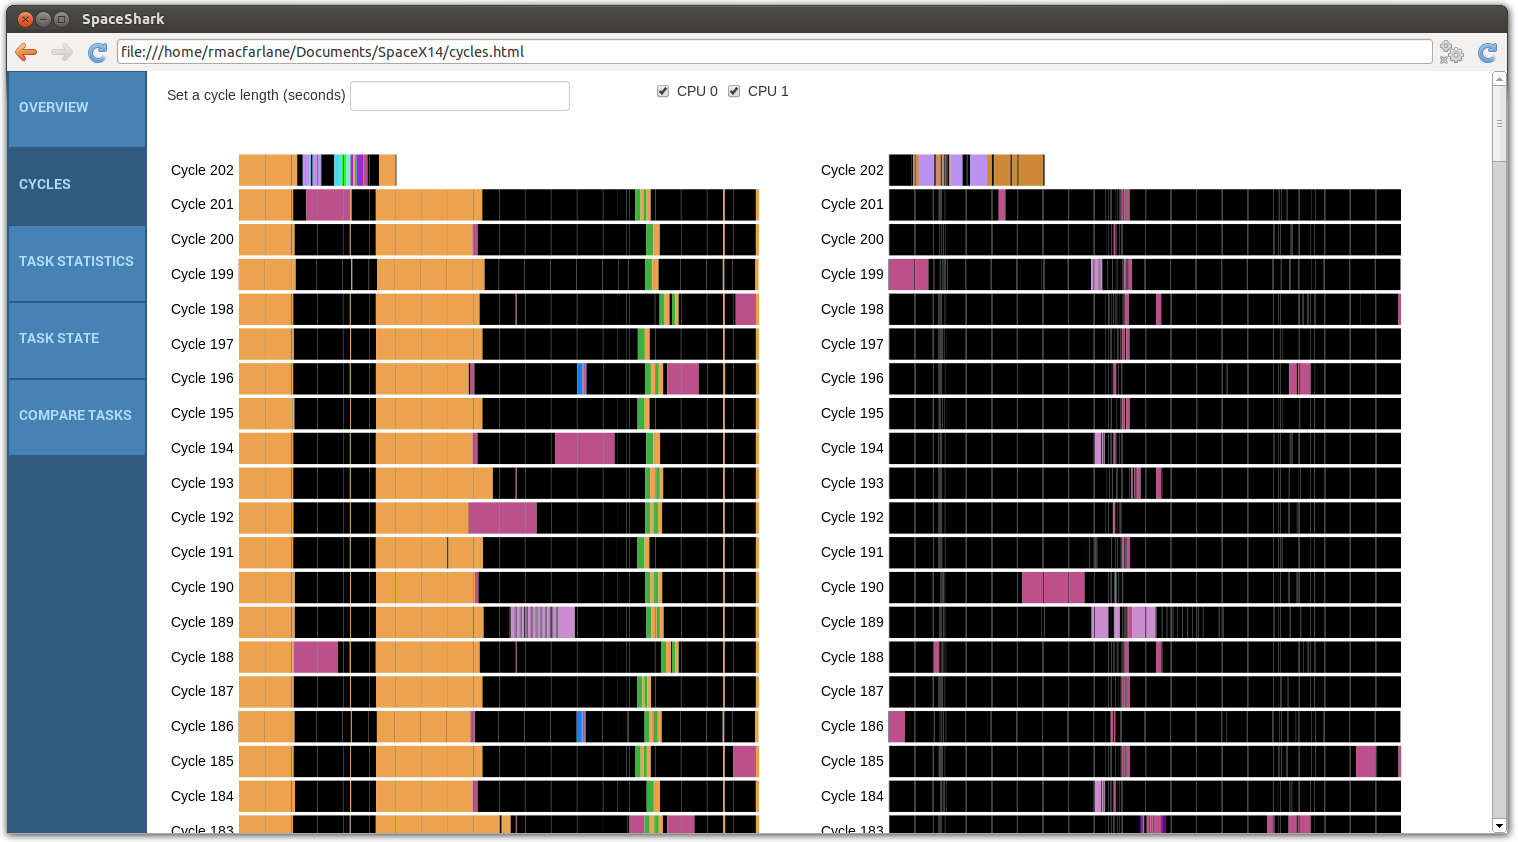
\includegraphics[width=5in]{cycles-page.png}
  \caption{The Cycles page displays graphs of each CPU. The user can define
  custom cycle intervals using the box in the top left. The checkboxes at the
top allow the user to select which CPUs to display.}
  \end{figure}
  
  \paragraph{Purpose:}Tasks run in cyclical patterns on SpaceX rockets, so being
  able to compare cycles helps find strange behavior. The Cycles page breaks the
  data into cycles and stacks them, allowing a user to easily scan down this
  graph for unusual behavior.

\paragraph{Interactivity:}    
    Like the graph on the Overview page, the user can zoom and pan the graphs on
    the cycles page.  The page also has checkboxes to toggle on and off each
    CPU, which removes or adds the graphs for these CPUs, rescaling other graphs
    to use the full window space. Cycle lengths are precomputed if the user
    included markers in their code to indicate where cycles start when data is
    collected.  If not, the graphs will not appear when the page first loads.
    The user can enter a number in the top box to set the period of desired
    cycles, which will then display a graph of cycles of that length. This
    feature also works  if print events are present in the data.  Entering a
    number at the top applies the change to all currently displayed charts.
        
\paragraph{Comparison to KernelShark:}
    KernelShark is a general-purpose tool. The average user does not run tasks
    in a cyclical pattern, so KernelShark does not have any features to handle
    cycles. Identifying cycles is critical to debugging at SpaceX.
    
  \subsection{Task Statistics Page} %May Lynn

  \begin{figure}[H]
  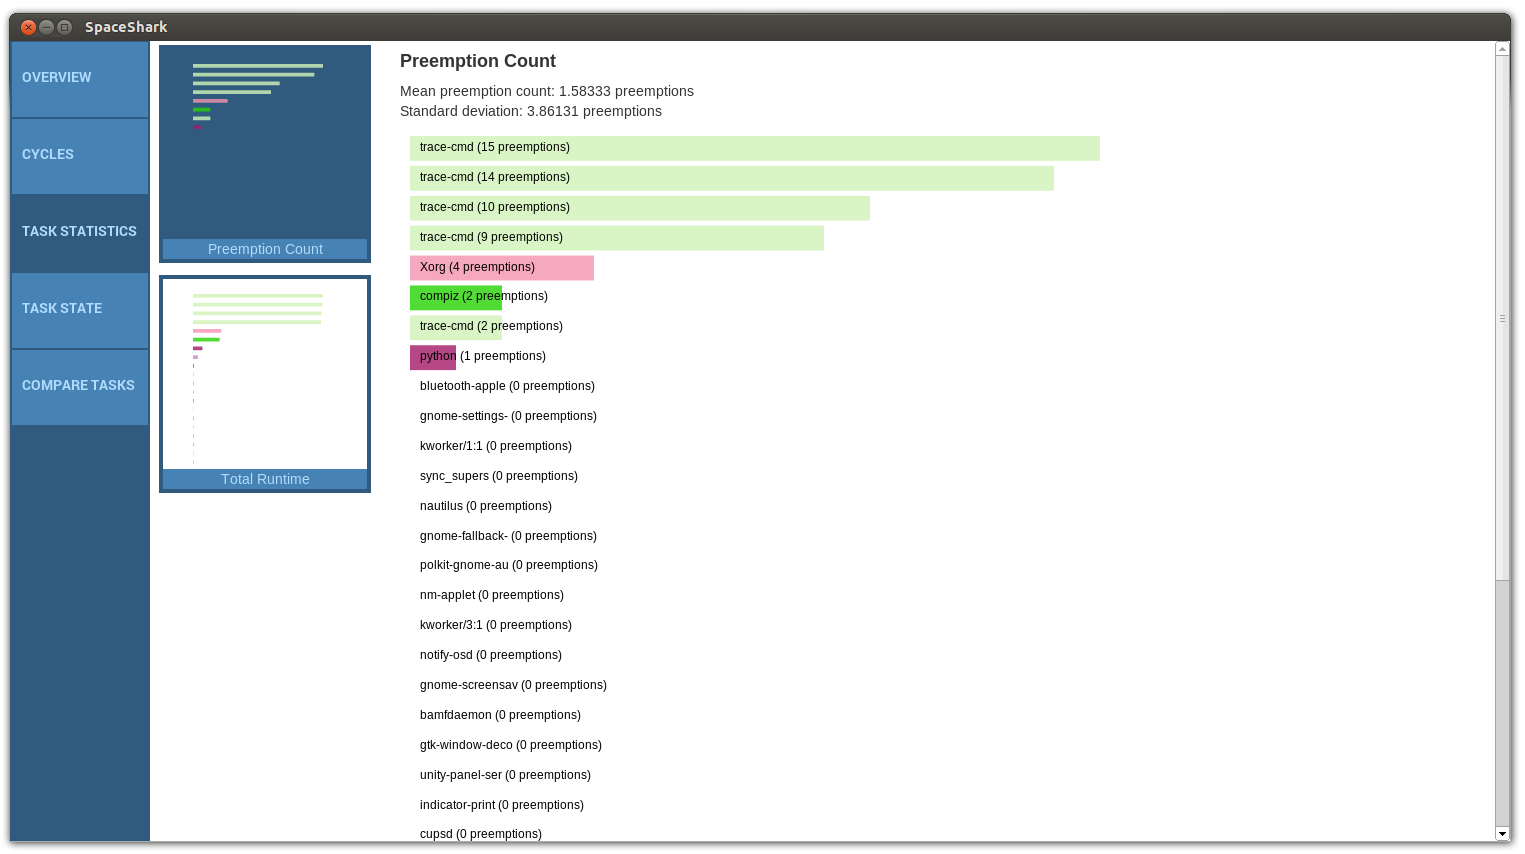
\includegraphics[width=5in]{task-statistics-page.png}
  \caption{The left column allows the user to navigate the bar charts, while
    also serving as a quick thumbnail view of each one. The right side displays
  the bar chart in a larger, more detailed view.}
  \end{figure}

\paragraph{Purpose:}
The Task Statistics page shows the number of times each task was preempted and
its total running time. This information is displayed in a bar chart sorted from
highest to lowest, with averages and standard deviations across all tasks at the
top. It is easy to see if there are any outliers with a large number of
preemptions or a long runtime.

\paragraph{Interactivity:}
All bars in the graph have distinct colors to represent different tasks. These
colors are consistent with the color scheme throughout the rest of the
application. The user can click on any task in the bar graph and will be
redirected to the Task State page for more information about that task.
The user can toggle between viewing the preemption count graph and the runtime
graph by clicking the small graph thumbnails in the sidebar.

\paragraph{Comparison to KernelShark:} KernelShark does not compute any
statistics about the data.


  \subsection{Task State}

  \begin{figure}[H]
  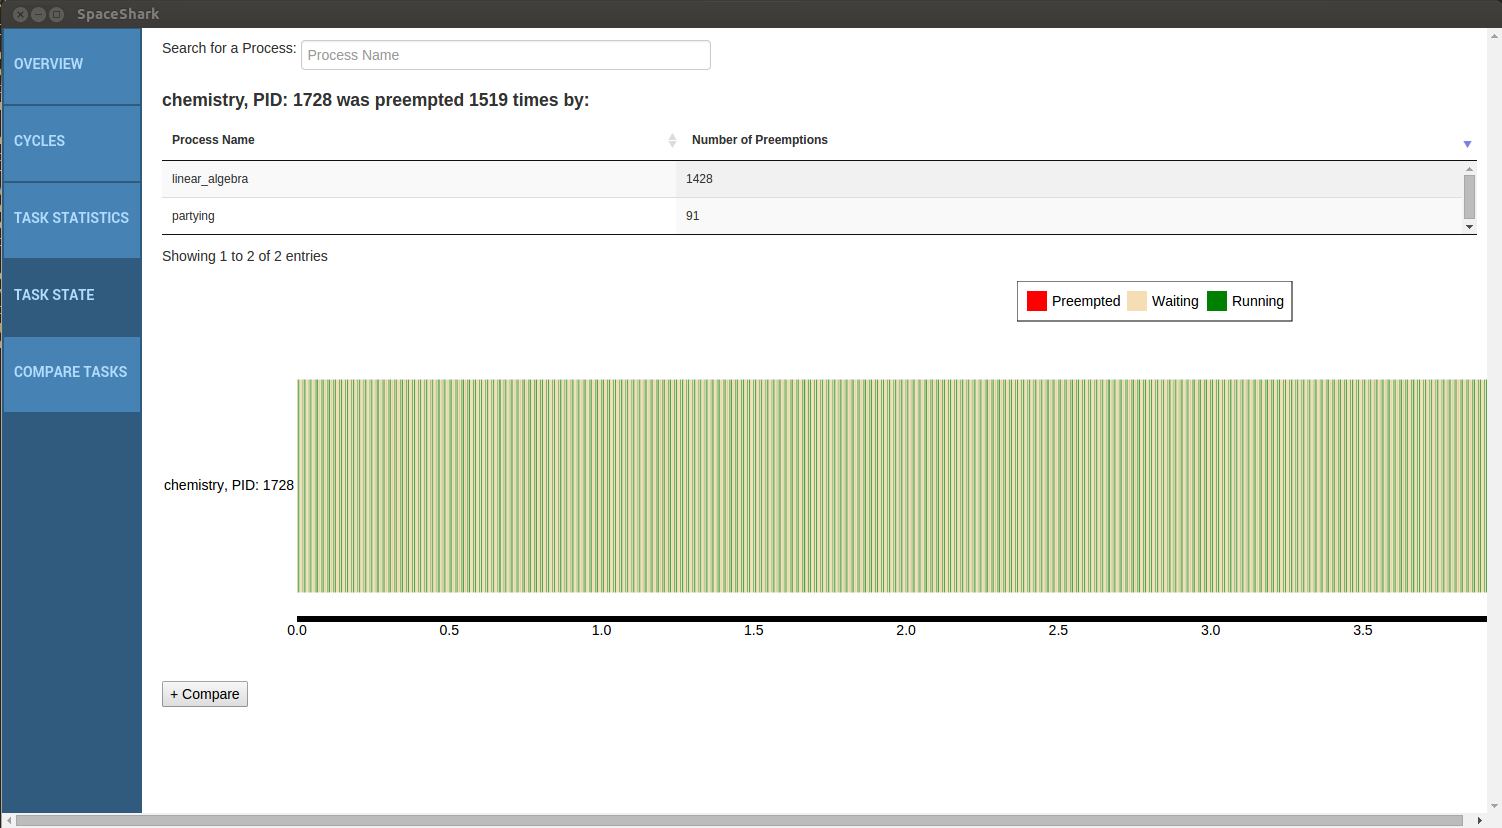
\includegraphics[scale=0.3]{task-state-page.png}
  \caption{The top of the Task State page displays a table of tasks
  that preempted the current task. The bottom half is a graph that plots the
state of the current task over time. The three possible states are preempted,
waiting, and running.}
\end{figure}

\paragraph{Purpose:}
    The Task State page displays information about a single task. The table in the top portion of the screen shows which other tasks preempted the task the user is viewing, and how many times. Users can jump to tasks that preempted the current one by
    clicking on a row in this table. Additionally, the task's state over time
    is displayed at the bottom. Possible task states are preempted, waiting, or
    running. They are labeled with the colors red, beige, and green respectively. 

\paragraph{Interactivity:}
    The graph on the bottom half of the page functions the same as the graphs on
    the Overview, Cycles, and Compare Tasks page
    . The user can click the ``+ Compare'' button at the bottom
    to add this task graph to a series of side-by-side graphs for comparison.
    
\paragraph{Comparison to KernelShark:}
     KernelShark can display a graph of a single task over time, however it does not show which other tasks preempted a given task, nor how many times it was preempted.
  
  \subsection{Compare Tasks} %Wendy
  
  \begin{figure}[H]
  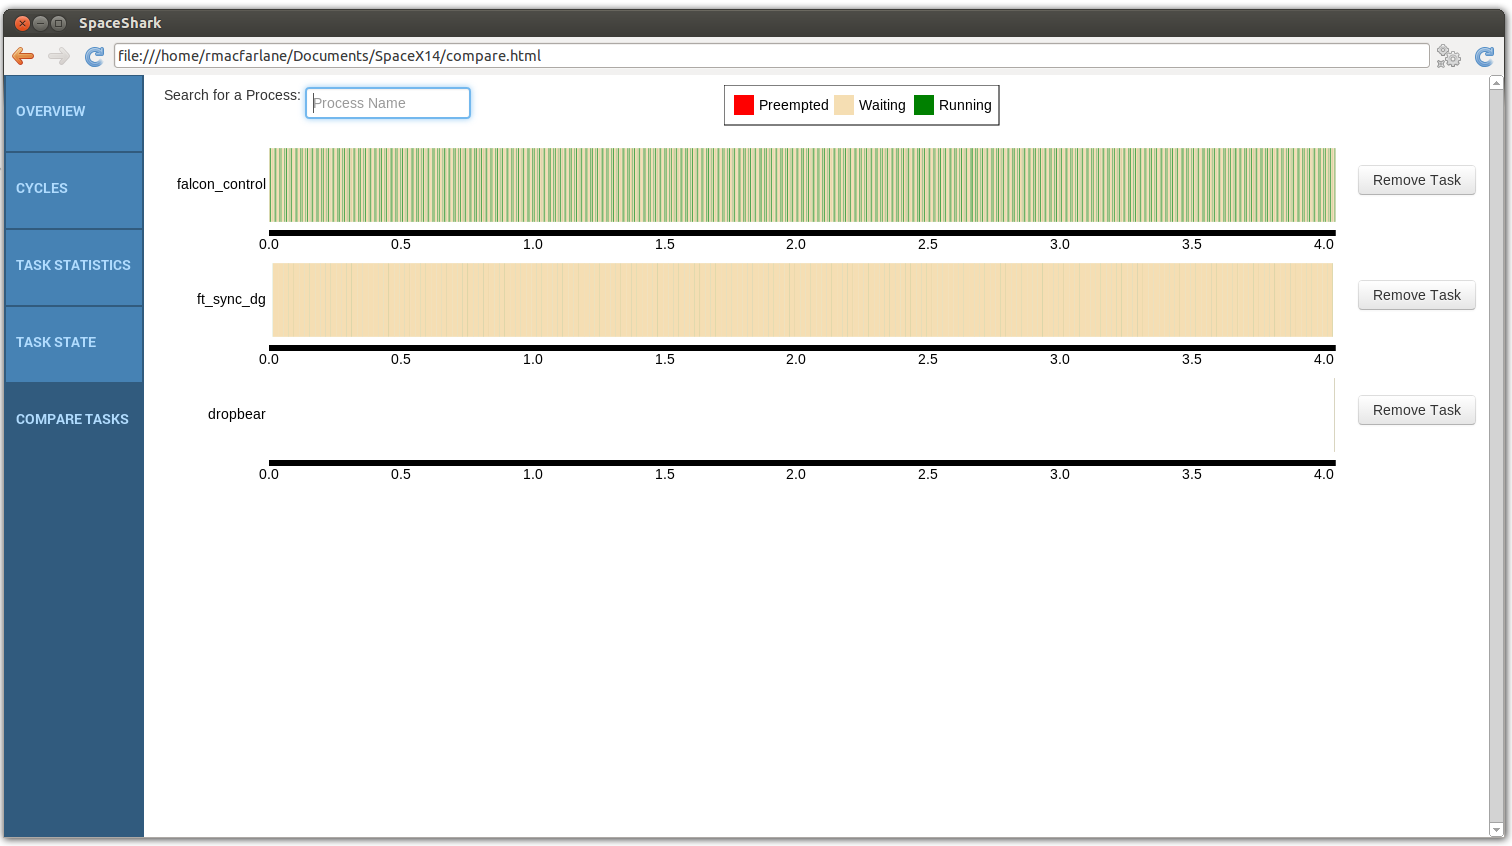
\includegraphics[scale=0.3]{compare-page.png}
  \caption{The Compare page vertically displays the Task State graphs for
  multiple tasks. They can be added, reordered, or removed.}
  \end{figure}

\paragraph{Purpose:}
The Compare Tasks page allows users to view the state graphs for multiple tasks. Tasks can be reordered so that specific tasks can
be compared side by side for the same time period. 

\paragraph{Interactivity:}
Users can plot graphs by either (1) typing in a task name or PID in an autocomplete box at the top of the page, or
(2) viewing a task on the Task State page and clicking the ``+ Compare''
button. The user can
rearrange the order of the graphs on the page by dragging them up or down. Each
graph can be removed by clicking on the ``Remove Task'' button next to it.
    
\paragraph{Comparison to KernelShark:}
    In KernelShark, the user can view a list of tasks and select which
    ones they want to graph.  This list of tasks is not searchable. In our tool,
    the autocomplete functionality we provide is much faster and easier than
    scrolling through a long list of tasks.

\chapter{Architecture}

\section{Introduction}
In this chapter, we describe the different components that form our application.
This information is useful for someone who wants to modify SpaceShark in some
way, for example by adding a new feature or making a change to the type of data that SpaceShark can display.

\section{Overview}

  Our application has three main components: the raw input, the parser,
  and the web-based desktop application. The raw input consists of information recorded on a computer that details what each task was doing for a short amount of time. The parser is a program that we wrote to translate this data into something that could be easily read by our application. The components are modular, and
  as long as output and inputs remain the same, internal changes to one section will
  not affect the others at all. In this chapter, we  discuss in more detail how each
  component works and how they come together to form a complete program.
  Figure 2.7 provides a visual representation of the flow of our application
  while also displaying its modular parts.
  
  \begin{figure}[H]
    \begin{center}
  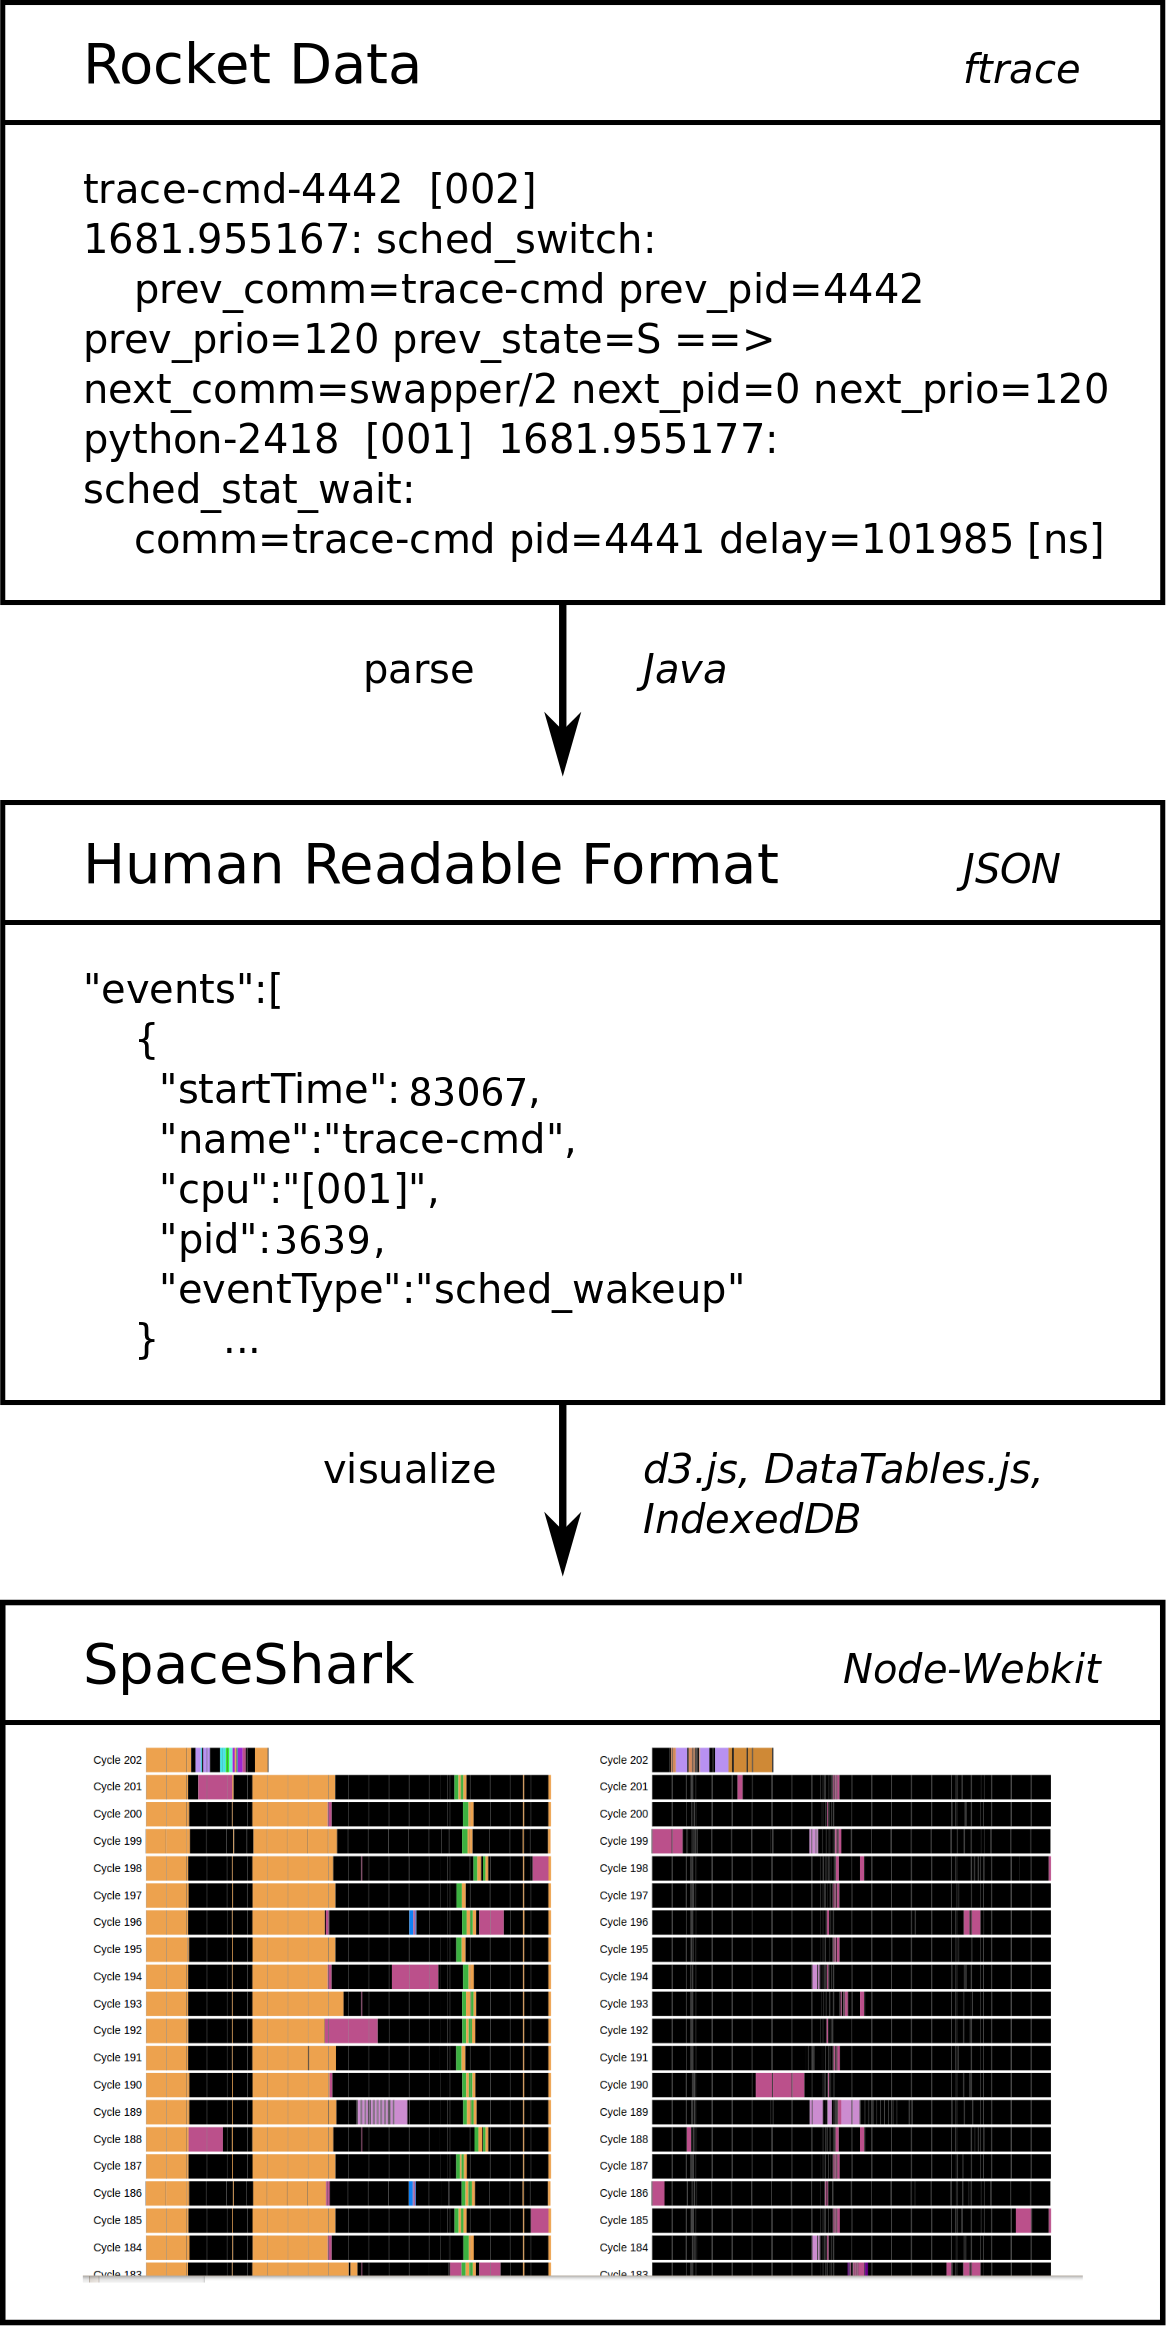
\includegraphics[scale=0.15]{architecture_diagram.png}
  \caption{A visual representation of three portions of our application. Each
  piece flows into the others while remaining modular, coming together to make our final tool.}
\end{center}
\end{figure}

  \section{Trace-cmd}

  Spacex engineers collect data using a command-line utility called \texttt{trace-cmd},
 which captures various events in the Linux kernel while it runs. The user specifies the kinds of events \texttt{trace-cmd} should record. SpaceShark users are interested in scheduling events: what tasks were
  scheduled to run, wait, and migrate between CPUs over the time of the trace.
  We therefore assume that the user has taken a trace that captures scheduling
  events.

  The \texttt{trace-cmd} utility can generate a human readable
  report of this record. An example line from a report is shown below.
  
\footnotesize\begin{verbatim}<idle>-0   [002]  2296.990243: sched_wakeup: comm=nautilus pid=2390 prio=120\end{verbatim}

\normalsize
  
% FIXME put in future work
%  The downside of this is that the format of the file generated by \texttt{trace-cmd
%  report} is dependent on the version of \texttt{trace-cmd} used. To be able to reliably
%  parse data and add additional information about preemptions, we need our input
%  data to have a consistent format. This creates a dependency on a particular
%  version of \texttt{trace-cmd}. The team has chosen to use \texttt{trace-cmd} version 2.2.1, 
%  the same version that our liaisons currently use.

  \section{Parser}
  Next the parser takes in this raw data, and ultimately outputs the data
  reformatted into JSON with additional information.

%% TODO this image is a little too low resolution
  \begin{figure}
  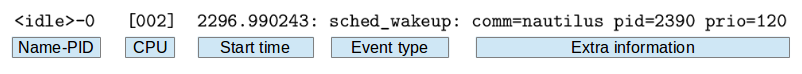
\includegraphics[scale=0.4]{parserExample.png}
  \caption{An example line of raw input, with the specific pieces labeled.}
  \end{figure}

  The fields that are recorded for each event are task name, PID, start time, 
  event type, and extra information. The fields are labeled in Figure 3.2. 
These five fields appear for every event, but the content of extra information
  varies based on the type of event.

  To parse these event lines, the parser reads the file line by line and breaks on
  whitespace. Then it is easy to extract fields one by one. To deal with the
  extra information field at the end, the parser cases on event type. Switch events
  are the only types of events that contain extra information that we need.  The
  extra information field of switch events gives the name, PID, and priority of
  the task being switched in for the currently running task. Importantly, it
  also contains a flag that indicates if the task being switched out transitions
  to a runnable or sleeping state. If the task is switched out and into a
  runnable state, it has been blocked, which means the event is a preemption.

  The parser also calculates the total runtime of each task by looking for
\texttt{sched\_stat\_runtime} events. These events give the time elapsed between
  a task being switched in and out of a processor, so by summing them for 
  each event, we are able to add a field to a task giving total runtime.

  The output is formatted as a JSON (JavaScript Object Notation) file, so that we can easily transfer it to
  the web application. The output JSON has the following elements:

  \begin{center}
    \begin{tabular}{p{0.35\linewidth}p{0.55\linewidth}}
      \toprule
      \texttt{Tasks}      & An array of all tasks seen in the trace\\
       \texttt{Events}     & An array of all events seen in the trace\\
       \texttt{cycleEvents} & An array of cycle events generated from user markers\\
       \texttt{numCPUs}     & Integer, how many CPUs were in the trace\\
       \texttt{AutocompleteNames} & An array of strings, listing all tasks names\\
       \texttt{AutocompleteEventTypes} & An array of strings, listing all event types in the trace\\
      \bottomrule
    \end{tabular}
  \end{center}

  As noted, several of these JSON objects contain other JSON objects: tasks,
  events, and cycleEvents. A task has the following data.

  \begin{center}
    \begin{tabular}{p{0.3\linewidth}p{0.2\linewidth}p{0.4\linewidth}}
      \toprule
      Field           & Type         & Additional description \\
      \midrule
       \texttt{name}            & string       & \\
       \texttt{pid}             & int          & \\
       \texttt{events}          & int array    & Indices into the Events array to find associated events\\
       \texttt{preemptedBy}     & string array & Names of tasks that preempted this task \\
      \texttt{preemptionCount} & int          & A running total of times this task was preempted                    \\
       \texttt{totalRuntime}    & long         & Time this task ran in milliseconds during the trace        \\
       \texttt{totalWaittime}   & long         & Time this task waited in milliseconds during the trace     \\
       \texttt{totalSleeptime}  & long         & Time this task slept in milliseconds during the trace\\
      \bottomrule
    \end{tabular}
  \end{center}

  An event contains the data in the table below. Switch events contain some additional
  information. The switch event itself belongs to the task that is being
  switched out, but in the extra information field we also note which task
  was being switched in.

  \begin{center}
    \begin{tabular}{p{0.2\linewidth}p{0.1\linewidth}p{0.6\linewidth}}
      \toprule
      Field     & Type   & Additional description                 \\
      \midrule
       \texttt{name}      & string &                                        \\
       \texttt{pid}       & int    &                                        \\
       \texttt{cpu}       & int    &                                        \\
       \texttt{startTime} & double & Time in milliseconds since kernel boot \\
       \texttt{eventType} & string &                                        \\
      \texttt{extraInfo} & string &                                        \\
       \texttt{activeName}* & string & The name of the task switching in      \\
       \texttt{activePID}*  & string &                                        \\
      \bottomrule\\
\multicolumn{3}{l}{ *This information is only present on switch events.}
    \end{tabular}
  \end{center}

 

  The \texttt{trace-cmd} utility can also pick up ``print'' events. Print events allow users to add
  their own markers as a task runs. A user can generate a print event by making
  an addition to the code of a task. We rely on these user-generated markers to
  identify cycles. Print events occur periodically in some of the tasks we are
  tracing. Engineers use print events already, so we check to see
  that the user has annotated them with \texttt{CYCLE\_START} by looking at the extra
  information field of a print event. If the extra information field starts with
  \texttt{CYCLE\_START}, then we create a \texttt{cycleEvent} that contains the following data.

  \begin{center}
    \begin{tabular}{lll}
      \toprule
      Field     & Type                \\
      \midrule
       \texttt{startTime}      & double                               \\
       \texttt{extraInfo}       & string                              \\
      \bottomrule
    \end{tabular}
  \end{center}

  To see an example of the JSON file, view Appendix A at the end of the report.
  \newline
  \newline
  
  Due to the modularity of our tool, the parser could be rewritten so long as
  the output format remains the same. Additionally, a user might have data
  in a format other than trace data. That user could write their own parser to
  convert their data into this JSON format. It could then be used in our tool.

  \section{Web Application}

  
  \subsection{Node-Webkit and HTML} %Rachel
    At the beginning of the project, the team researched possible tools and
    technologies for creating our application. One possibility was simply
    extending KernelShark, the existing tool. After looking at the code for
    this, a large number of C files, we decided it would be faster to
    reimplement and extend it in something else. Understanding the KernelShark code base
    would take a very long time, and there was very little documentation. This
    would allow us to more effectively use our time creating new features rather
    than working our way through an old code base. We
    looked into Java UI libraries for desktop applications, as well as
    web-technology based charting libraries.  We found node-webkit, which allows
    HTML/CSS/JavaScript applications to be packaged and run as desktop
    applications with no reliance on the internet. 
    Using node web-kit allowed us to take advantage of many existing UI widigits
    and charting libraries. Instead of spending time creating our own
    visualizations, we were able to quickly modify existing ones. This allowed
    us to devote more time to developing new and useful ways to view the trace
    data.

  \subsection{Primary JavaScript/CSS files}
  One of the primary JavaScript files we've worked
  with and changed is \texttt{gantt-chart-d3.js}. This file contains the logic for all of the
  graphs. This file was originally written by Dimitry Kudrayvtsev, %% TODO add a reference?
 but we have significantly modified it to produce the behavior we want.

  The graph takes in data and groups it by a particular attribute. Each piece
  of data, here, a scheduling event, is rendered as a rectangle. The
  length of the rectangle is determined by the event's duration, and its
  placement on the graph by its start time and group. Examples of groups are
  CPU or cycle.

  The graph assigns CSS classes to each rectangle so that they can easily be
  colored and sets up a mouseover handler to display hover text
  over an individual event. On the Overview page, clicking
  on an event will scroll to it in the data table.
  Lastly, we added zooming behavior to the chart that is
  preserved on navigation. By using Local Storage, the application is
  able to check that charts added to the compare page will render at the
  same zoom level as others, and will zoom in sync with one another.

  To function properly, the chart needs a list of events
  as well as a property to group on. Behavior on each pages varies
  slightly, so a parameter is also passed to indicate to the chart the page on
  which it is rendered

  The file \texttt{sidebar.js} is a script that creates the sidebar for all of the
  pages, excluding the first page of the application where the user chooses a file.
  This script controls navigation and sets highlighting of the current tab.

  Below is a list of the libraries the application uses with links to
  their respective sites, which include documentation.
\begin{itemize}
\item d3.js (d3js.org)
% d3 - http://d3js.org/
\item dc.js (dc-js.github.io/dc.js)
% dc - http://dc-js.github.io/dc.js/
\item Draggabilly (draggabilly.desandro.com)
% draggabilly - http://draggabilly.desandro.com/
\item Packery (packery.metafizzy.co)
% packery - http://packery.metafizzy.co/
\item DataTables (datatables.net)
% datatables - https://www.datatables.net/
\item Twitter Typeahead (twitter.github.io/typeahead.js)
% typeahead - https://twitter.github.io/typeahead.js/
\item Underscore (underscorejs.org)
%% FIXME - any more?
\end{itemize}

  \subsection{IndexedDB}

  The application loads the JSON file into IndexedDB, a
  browser-based database. IndexedDB is built into most browsers, including
  node-webkit, which runs Chromium. More information on the details of IndexedDB can be found here:
\begin{center}
  https://developer.mozilla.org/en-US/docs/Web/API/IndexedDB\_API
\end{center}
  We use IndexedDB to store data so that it does not have to be reloaded every time the user navigates to a different page. It also
  maintains storage between application sessions.
  Specifically, the application stores:
  \begin{itemize}
    \item \texttt{numCPUs} (number of CPUs for this file)
    \item \texttt{cycleEvents} (the events partitioned into cycles for the Cycles page)
    \item \texttt{Tasks} (a list of all the tasks with various information)
    \item \texttt{AutocompleteNames} (used for autocomplete in search bars)
    \item \texttt{AutocompleteEventTypes} (also used for autocompleting)
    \item \texttt{Events} (a list of all the events)
  \end{itemize}
  These correspond to the JSON types laid
  out in the Parser section (Section 2.2.3).


%  Using the node-webkit profiling tool, we can see that IndexedDB is the slowest
%  part of our application, as transactions with the database must be opened and
%  closed. Ideally, we would use something less complex, but other options such
%  as Local Storage did not have enough space for our large files.

  IndexedDB also has  a size limit, but this is typically not reached except for
  unusually long files or data from a computer with many CPUs. 

  \subsection{Local Storage}

  SpaceShark also makes use of Local Storage, another tool
  built into most browsers and node-webkit. This is a small and quick-to-access
  storage method. We primarily use it to save state between pages, notably
  display states. One example is the zoom level of the graph, which does not
  change between loads of the same page. Local Storage is also retained between
  application sessions.

  SpaceShark stores the following information in Local Storage:

\begin{itemize}
  \item \texttt{cellData}: A string containing the name and PID of the task currently being
  shown on the Task State page. 
\item \texttt{compareCurrScale}: The last recorded scale for the Compare Tasks graphs.
\item \texttt{compareCurrTranslateX}: The last recorded x translate for the Compare Tasks
  graphs.
\item \texttt{compareData}: A list containing strings with the names and PIDs of the
  tasks currently being shown on the Compare Tasks page.
\item \texttt{cyclesCurrScale}: The last recorded scale for the Cycles graphs.	
\item \texttt{cyclesCurrTranslateX}: The last recorded x translate for the Cycles graphs.
\item \texttt{displayedCPUs}: A list of the CPU numbers that are being displayed on the
  Cycles page.
\item \texttt{firstEventTime}: The time that the first event occurs, before we
  normalize the events to start at 0.
\item \texttt{hasEverExisted}: SpaceShark checks this variable to see if there
  is content in Local Storage. If it exists the user is given the option to use
  their previous data on the Load File page.	
\item \texttt{mainCurrScale}: The last recorded scale for the Overview graph.	
\item \texttt{mainCurrTranslateX}: The last recorded x translate for the Overview graph.
\item \texttt{maxDuration}: The longest time in seconds that a CPU ran for. Serves as
  the end time for all graphs.
\item \texttt{processCurrScale}: The last recorded scale for the Task State graphs.
\item \texttt{processCurrTranslateX}: The last recorded x translate for the Task State
  graphs.
\item \texttt{tableScroll}: Used by the Overview table.
\end{itemize}
\texttt{DataTables.js}, a package we use, also makes use of Local Storage in order to save the scroll position of the table.

  \subsection{Overall Application Structure}

  The general structure of our code is similar to most web applications. 
  The root directory contains HTML files, which reference JavaScript and CSS files. The files
  we have written are located in \texttt{assets/js} and \texttt{assets/css}, and
  library files reside in \texttt{lib/js} and \texttt{lib/css}.  Each page has
  its own JavaScript file, and there are a number of shared SpaceShark files that
  multiple or all pages use.
  

  \begin{center}
    \begin{tabular}{p{0.2\linewidth}p{0.7\linewidth}}
     \toprule
      Page Name       & Code artifacts     \\
      \midrule
      Load File       & \texttt{assets/js/loadFile.js}\\
      Overview        & \texttt{assets/js/main.js, assets/js/gantt-chart-d3.js, dataTables.js}\\
      Cycles          & \texttt{assets/js/cycles.js, assets/js/gantt-chart-d3.js}\\
      Task Statistics & \texttt{assets/js/runtimeChart.js, assets/js/preemptionChart.js}\\
      Task State      & \texttt{assets/js/process.js}\\
      Task Compare    & \texttt{assets/js/compare.js}\\
    \bottomrule
    \end{tabular}
  \end{center}

  \subsection{Selection of Charting Tool} % Rachel
  Many pages render a timeline of running tasks that users can interact
  with by panning and zooming. This graph is critical, as a bug on the rocket manifests
  itself as a task running at an unexpected time, or failing to run at a
  particular time. We spent several weeks experimenting with different
  JavaScript charts, including \texttt{timeline.js}, \texttt{vis.js} and
  \texttt{gantt-chart-d3.js},
  to find one that would be suitably fast and easy for us to add new
  features to. Our main selection criteria were speed, zooming and dragging
  capabilities, and either built-in or easy-to-add handlers for user clicks
  on portions of the chart. We decided to use \texttt{gantt-chart-d3.js} because it
  renders more quickly and is more responsive than the other charts. It
  also comes with dragging capabilities, and hovertext and
  click handling could easily be added. Zooming on d3 charts should be
  available out of the box, but did not function as expected because our y scale
  is ordinal rather than numeric and should not be rescaled. The team
  ended up writing a custom zoom function to handle this and other issues
  associated with syncing the zoom level of multiple charts on the same page.
  
  \subsection{Creating a Timeline}
  On the Overview, Cycles, Task State, and Compare Tasks page, the same type of
  graph is used. The graph shows either which task is running at a given time,
  or what state a task is in at a given time. The graph is fed a list of
  events to display and a number of optional settings before being drawn. The
  array of all events needs to be passed through several helper functions
  before it is ready to be given to the graph.
  
  \begin{enumerate}

    \item The events list is filtered to only contain switch events. Switch
      events indicate that one process switched out, either by preemption or
      because it finished.
      Switch events are all that are needed to determine which task was running, or
      what state a task was in.
  
    \item All start times are normalized so that first event is at time zero.
      In the original events list, the start times of events are given in
      milliseconds since kernel boot, which is not relevant. We separate our
      events by CPU, and for each grouping of events, shift the start times
      so that the first event occurs at time zero.
  
    \item The graph requires a time domain as in input, so the endpoint of the
      last event is calculated.
      How this calculation is performed depends on which page the user is
      on. On the Overview page, this comparison is across all CPUs. Each CPU may not
      be processing tasks for the entire duration of the trace. For example, all
      events on CPU 0 might take only three seconds, while all events on CPU 4 take
      four seconds. We take the maximum of the total duration of events across CPUs, in our
      example, four seconds. The same calculation is used for the compare page so
      that the time range on the x-axis will be the same across all tasks.  On
      the Cycles page, our time range is simply the length of a cycle.
  
    \item The Gantt chart is passed its parameters in preparation to be drawn,
      not including the events. These parameters include the name of the page it
      is currently on, which will allow the chart to modify its behavior based on
      context, as well as what attribute to group by (CPU, cycle, or nothing).
      Width and height can also be passed, which allows charts on the compare
      page to take up little vertical space, while the Overview page chart uses
      as much space is available to it.
  
   \item The events have their duration calculated, to determine the size of
     each drawn
     rectangle. For example, the Overview page calculates the
     difference between the start times of consecutive switch events. This
     calculates the amount of time each task was running for.
  
   \item The Gantt chart is passed the events and drawn, and the colors are set.
     The chart assigns a CSS class to each task based on its PID, and randomly
     selects a color for this class and adds a style tag to the page. The random
     color selection is seeded so that the same colors will be assigned every
     time. We considered producing a stylesheet after parsing so the CSS did not have
     to be generated each time, but in profiling the application we saw that
     this process was actually quick, and decided this change was low
     priority.

  \end{enumerate}


\chapter{Winter Break User Feedback} % Alix
\section{General Feedback} % Alix
We sought user feedback about our designs and tool throughout the course of the
semester. Most of our feedback was from our liaisons, who we communicated with
on a weekly basis. The team was also able to user test with four SpaceX
engineers during a week long site visit at SpaceX. It was especially useful to
have people unfamiliar with our tool use it.  User testing helped the team
identify what features were useful, what features should be modified, and what
features needed to be added to make the tool as effective as possible.  We will
focus mostly on the negative feedback, both from our liaisons and user testing,
as critical feedback was the most useful in moving our tool forward.

Below we will cover our methodology of user testing, feedback for specific
pages, and how that feedback shaped the changes we made, leading to the current
version of SpaceShark.

\section{Methodology} % Wendy
User testing was conducted with four SpaceX engineers who all had some
experience using KernelShark. Testing was conducted with one subject
at a time over a half hour period.

During testing, two members of our team watched the user work their way through
our tool using our sample data, or in some cases the user's data if they had
some prepared. We tried to provide as little input as possible, except for
encouraging the team member to think out loud, describing what they were
expecting or doing, and why. While the user did this, we took notes on what they
were saying and doing.

Once the user felt like they had explored the tool, we talked more in-depth
about their experience, also elaborating on our intent with the tool,
encouraging explicit feedback on how we could make the tool better. A large
portion of this process went to brainstorming with the user and finding out why
a page was helpful or unhelpful for their specific workflow.

\section{Feedback on Specific Pages} % Alix

\subsubsection{Overview Page}

The main page of KernelShark featured a graphical display of the processes
running over time and a tabular version of the same information.

Before winter break, our tool also featured a graphical representation of tasks
running over time. The tool also displayed the top ten preempted, longest
running, and longest waiting tasks in tables at the top of the page. 

During user testing, three out of four users said that they did not find the
tables at the top of the page helpful. Two of the users described the typical
workflow they used in KernelShark as visually finding the problem in the graph,
jumping to that event in the events list, and then scanning the events list.
They felt that being able to quickly scan the events list was a very valuable
feature.

Based on this feedback, we removed the tables at the top of our page and added
an events list for users to interact with.

\begin{figure}[H]
\begin{center}
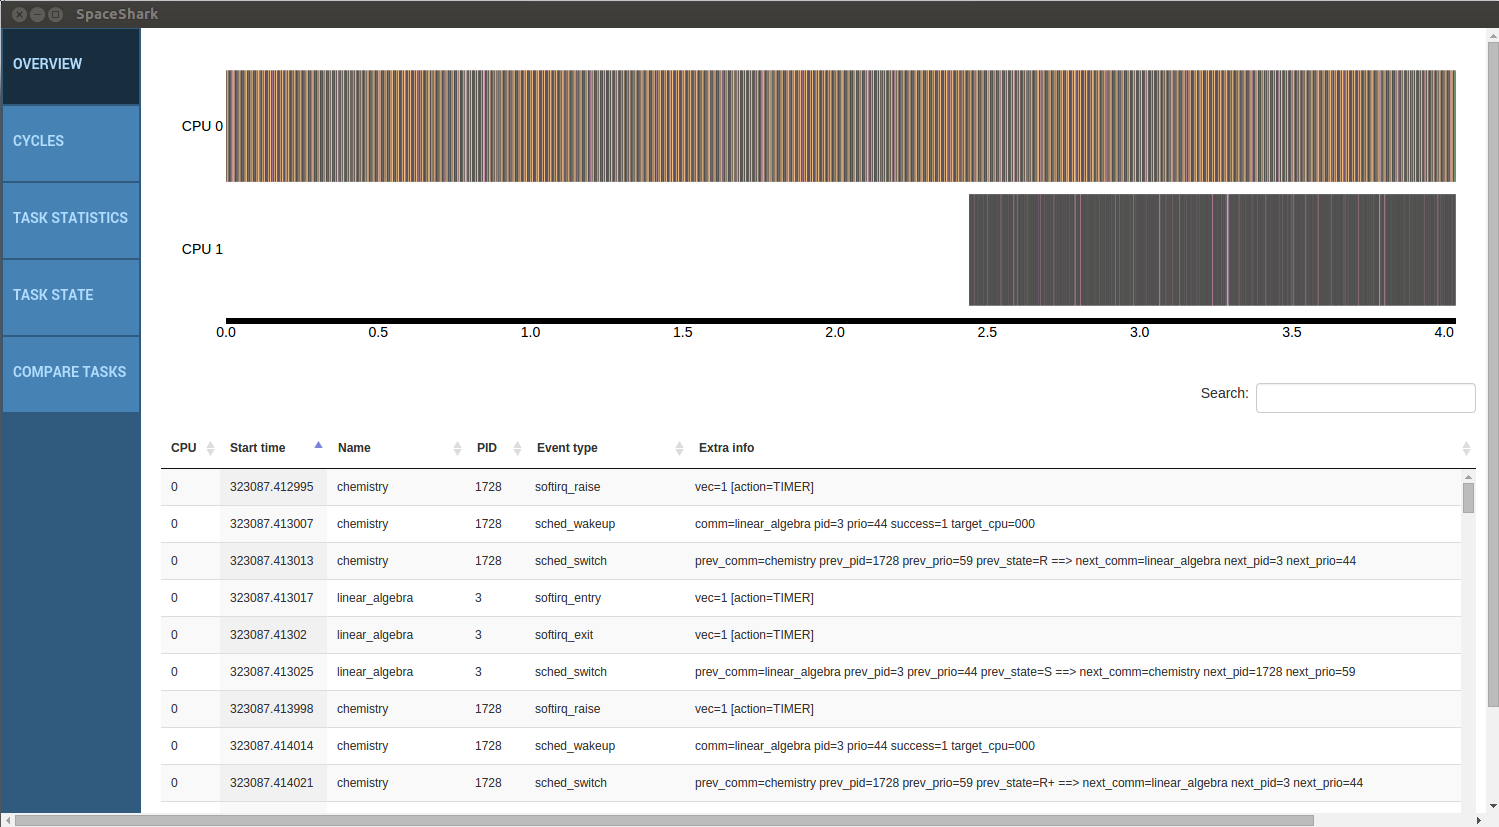
\includegraphics[width=4in]{overview-page.png}
\caption{A current screenshot of our Overview page. At the top is a graphical
representation of the tasks, and the bottom is a tabular view.}
\end{center}
\end{figure}

\subsubsection{Task State Page}

With KernelShark, a user could choose individual tasks to display under
the main timeline of all events. However, that was the extent of what
Kernelshark did with regards to individual tasks.

The team was interested in providing more details and statistics about
individual tasks. This would give users a different way to view
their data, which our liaisons thought would be helpful
in the debugging process.

\begin{figure}[H]
\begin{center}
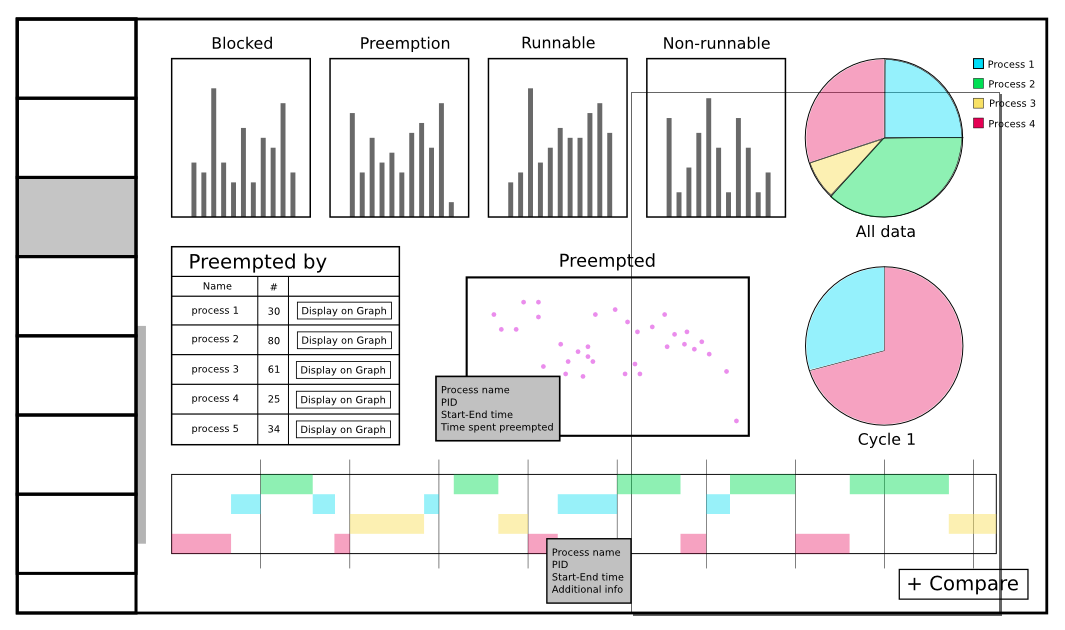
\includegraphics[width=4in]{perProcess-49.png}
\caption{The first mock-up we created for the Task State page.}
\end{center}
\end{figure}

Since there was no existing Task State page, we designed a mockup of it at the
beginning of the project. It features many different kinds of visualizations,
such as histograms of how long the task was in each state for, a scatterplot of 
what preempted it, a table of what preempted it, pie charts representing the 
data in cycles, and a graphical display of the time series data highlighting 
the process in the graph. Through user feedback with the liaisons, we found 
that our mockup included way too much information that SpaceX engineers would 
not have found useful. Since preemptions are generally
indicative of problems, we really wanted to focus on this on the Task State
page.

\begin{figure}[H]
\begin{center}
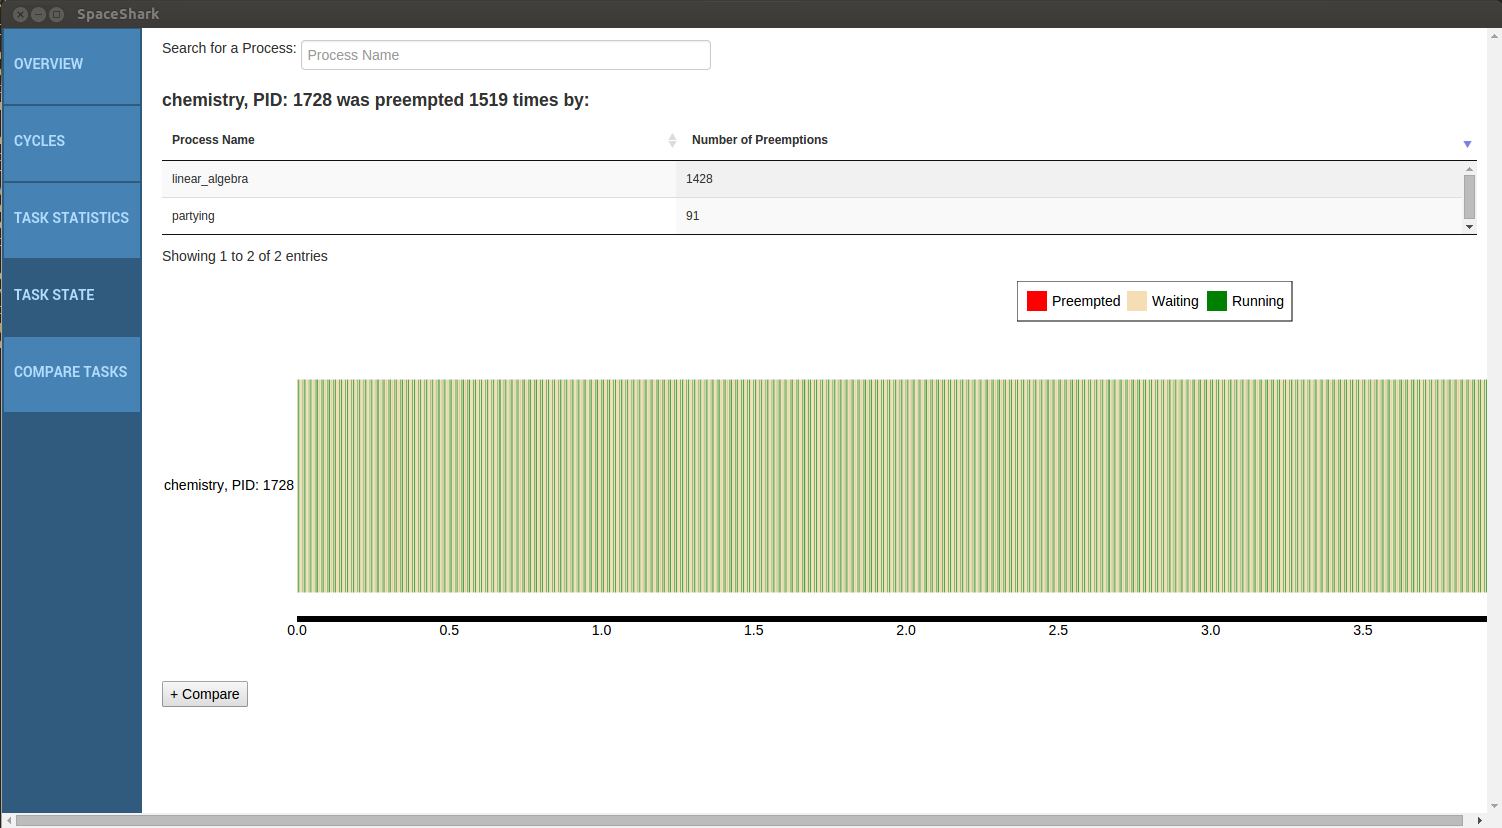
\includegraphics[width=4in]{task-state-page.png}
\caption{A screenshot of the current version of the Task State page. The three
colors indicate the three states a task can be in: running, waiting, or blocked.}
\end{center}
\end{figure}

On the Task State page, the user is able to type in a particular task, see
how many times it was preempted and which processes preempted it, as well as
view a graph showing how long it was in one of three states: running, waiting,
or preempted. This design has a minimalistic page view compared to the mockup,
but makes better use of the information it provides, and includes less
extraneous, unhelpful information.

This pages allows SpaceX engineers to find information on specific tasks, which
is something that KernelShark was unable to do. It helps engineers dig in to the
details, especially when used in conjunction with the broader context provided
on the Overview page and other pages.

When user testing, we received feedback that this page needed more context,
prompting us to create the Compare Tasks page. The Compare Tasks page has not
yet been user tested, but we hope it will meet this need by allowing users to
display multiple state graphs side by side to look at anomalies in context.

\subsubsection{Cycles Page}

One of the most notable things that separates our tool from KernelShark is that
KernelShark did not provide information about cycles, meaning that users had to
manually determine where cycles were.
The Cycles page in our tool lets the user easily find anomalies by splitting up
the Overview page graph visualization into cycles.

\begin{figure}[H]
\begin{center}
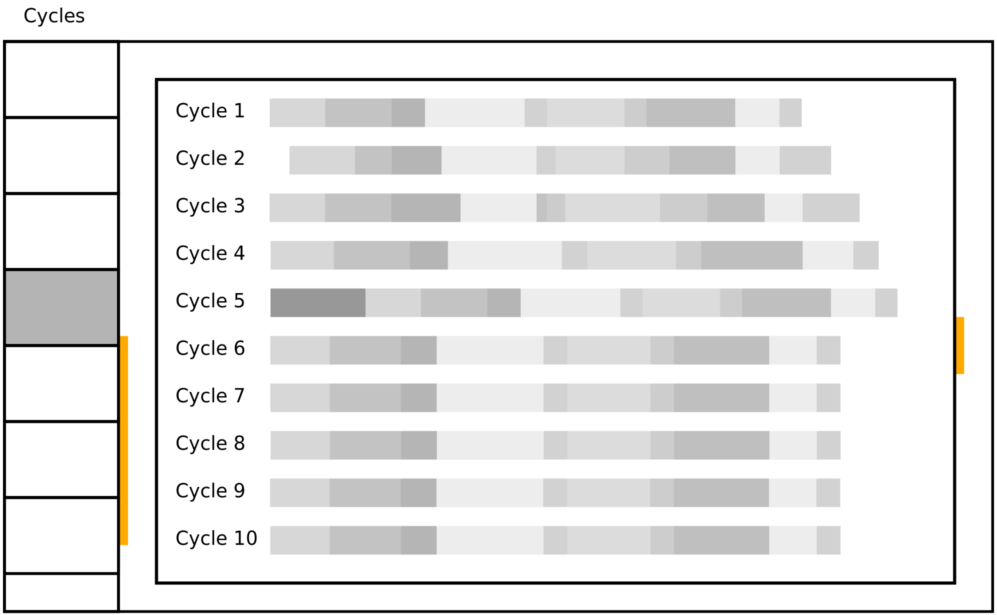
\includegraphics[width=4in]{oldcycles.png}
\caption{A mock-up of the Cycles page. Initially only one CPU at a time could be
displayed, as shown here.}
\end{center}
\end{figure}

We received nearly all positive feedback on the Cycles page, and this seems to
be the most useful aspect of our tool.

The first change  we made was very minor; rather than ordering the cycles from first cycle to last cycle, we changed it to be ordered from last cycle to first. We made this change because anomalies are normally found within the last cycle, which SpaceX engineers would want to see displayed prominently at the top of the page.

Additionally, this page initially relied on the user's code generating ``cycle
markers'', which meant that this functionality would not have worked with old
traces, or traces that didn't conform to our specific markers. One engineer
suggested that we add the ability to enter in cycle length and have it display
cycles based on that. We chose to implement this, taking this page from having
very specific requirements to being usable with any data.

\begin{figure}[H]
\begin{center}
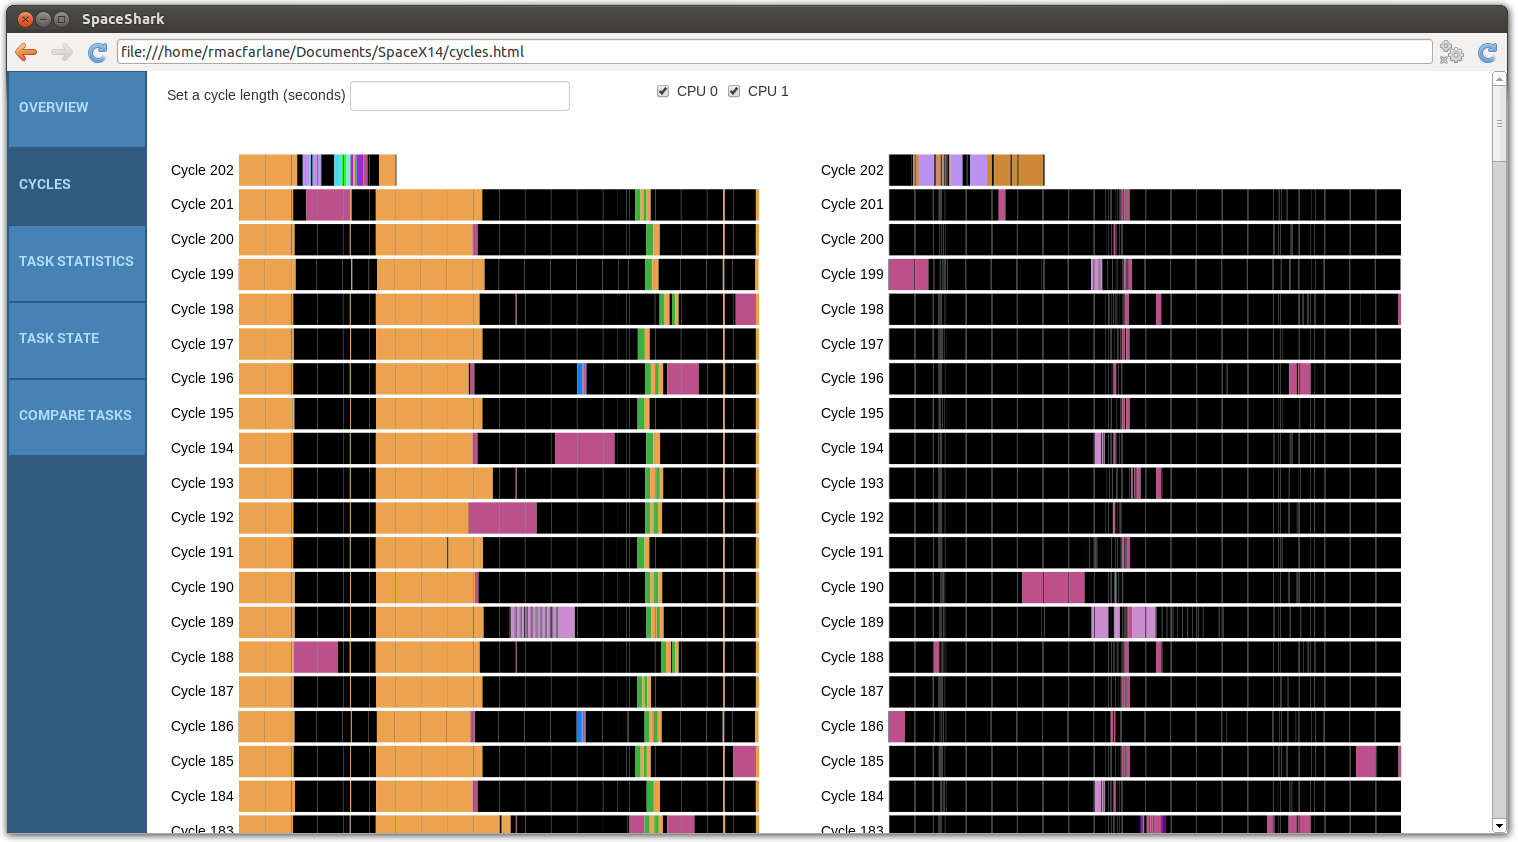
\includegraphics[width=4in]{cycles-page.png}
\caption{A screenshot of the current Cycles page. Multiple CPUs can be displayed
at once using the checkboxes at the top of the screen. The input box on the top
left allows users to choose their own cycle length.}
\end{center}
\end{figure}

%\chapter{Challenges}
%\section{trace-cmd versioning} % Rachel
%  As already described, we collect data using a command-line utility called
%  trace-cmd. trace-cmd records various events in the Linux kernel while it runs
%  and then outputs this information into a data file with a particular binary
%  format. trace-cmd also has a ``report'' option, which takes an existing trace
%  file and generates a human readable report of this record. Using this format
%  as a starting point instead of the raw binary format simplifies parsing.
%  We decided to leverage trace-cmd report instead of wrestling with the binary
%  data ourselves. This allowed us to make progress faster and to avoid working
%  on an already solved problem.
%
%  Unfortunately, the format of the file generated by trace-cmd report is
%  dependent on the version of trace-cmd used. For example, the formatting of the
%  ``extra info'' field of a switch event is liable to change. We use this
%  field to identify preemptions. To be able to reliably parse data and add
%  additional information about preemptions, we need our input data to have
%  a consistent format. This creates a dependency on a particular version
%  of trace-cmd. Our liaisons have been using trace-cmd version 2.2.1, so
%  our parser expects input data to be in the format of 2.2.1.
%\section{Selection of charting tool} % Rachel
%  We chose to use web technologies because we felt there was a wealth of
%  charting and UI/UX tools that we could use. We spent several weeks
%  experimenting with different charts for the main page. The main page renders a
%  timeline of running tasks, which is essentially a large number of colored
%  bars. This chart needed to be responsive to zooming and dragging, and to
%  dealing with click events to move to a particular time in the table of events
%  displayed below it.
%\section{Speed} %Wendy
%The data SpaceX will be using with our tool is very large, and becomes even
%larger once we have parsed it. As a result, some parts of the tool load slowly,
%and this is something we are still working on fixing. One main fix we have
%implemented is batch loading the list of events on the main page so that the
%user can start interacting with the tool without waiting to load the entire
%table, especially since all of the table is typically not needed.
%
%Having done some profiling, we know that pulling data from IndexedDB is the
%slowest part of our application, but at this point in time we do not have a way
%to fix this.

\chapter{Spring Semester User Feedback}
\section{Methodology}
   For this session, three members of our team attended the user testing sessions.
   We were able to test with three SpaceX engineers with differing levels of
   experience with KernelShark, so we received feedback from multiple perspectives.

   The users were instructed to read our README page on our GitHub page. They
   opened the application according to the instructions they read and were
   instructed to describe what they were doing out loud, why, and if they felt
   like anything was missing. As in our first round of user testing, the team
   provided little input while the user explored the tool using our sample data.

   This feedback session was after the clinic code freeze, so we were unable to
   implement the changes suggested. In the next sections, we will describe the
   suggestions and feedback, and detail how we would implement these where
   possible. We will start with feedback that is applicable to the application
   overall, and then discuss feedback for specific pages.

\section{General Feedback}

One noticeable missing feature was a list of all tasks for the user to view and select from. 
This would be best to add as an option on pages that require the user to select tasks, such 
as on the Task State page and the Compare Task page. It could appear as a dropdown menu or a 
pop-up dialog with checkboxes next to the names. It should be possible to sort these lists 
alphabetically or by pid as the user desires. The full list is especially suitable for the 
Compare Task page because it would allow the user to load multiple graphs at once. It should 
not be difficult to implement, as the tool already creates this list in 
\texttt{assets/js/compare.js} and \texttt{assets/js/process.js}.

We received a lot of feedback regarding the graph, including bug fixes and adding new functionality.
  \begin{itemize}

  \item The labels associated with the graphs should be static, and not go off the screen when 
  the graph is zoomed or panned. This is especially problematic on the Compare Tasks page, 
  where the user will potentially have large numbers of graphs displaying, and it will be 
  important for them to not have to remember what each graph is displaying.

  \item User testers found that they often had trouble or could not see smaller events 
  from the fully zoomed out view. This makes it harder to find trouble spots. We do not 
  have any suggestions on how to fix this, but it is an important issue that should be 
  considered.

  \item User testers were very interested in having the ability to place markers, which 
  is something that KernelShark implemented. The user should be able to place one or two
   vertical line markers onto a graph by clicking. If two markers are placed they should
    be able to get the duration between the two markers, and shift the two markers as one
     unit over the graph, maintaining the same duration between them. The markers could
      potentially be added to the graph at the SVG level, which would likely mean they 
      would pan with the graph as desired, although zooming would require some extra 
      work to keep the markers as a thin line.

  \item User testers often had trouble distinguishing where using the mouse scroll wheel
   would zoom in on the graph, and where it would scroll down the page. One potential fix
    for this is to make it more clear where the graph is by changing the white background
     to be a light, desaturated color or a light grey. This would make the
     graph's ``white
      space'' distinguishable from the page, making it easier for the user.

  \end{itemize}

One user was very interested in the idea of exporting the state of the tool. One 
potential way we could do this is to write the state (via the local storage variables)
 to the end of the JSON file, and have a check when we load files to see if there 
 is a state to load. This would potentially be very difficult, as we are not sure 
 that JavaScript would allow you to write to a file. The benefit of being able to 
 export the state hinges around the idea that it would be easier for a user to 
 share their findings with other people. A user receiving this data would have the 
 information in the same state as the original user, eliminating time spent walking 
 through the data to find the desired information. It would also allow the user to 
 work from multiple computers.

\section{Overview Page}
One user suggested that the graph respond when an event in the events list is clicked.
 This would mirror the existing behavior of clicking on an event in the graph and having
  it scroll in the events list. One possibility for how the graph could respond is adding
   a marker at the timestamp of the event clicked onto the graph. A second possibility is
    translating the graph so that this event is now at the left. Lastly, the graph could 
    be translated so that the event is in the center.

  To translate the graph, the $x$-position of the switch event closest in start time to
   the event clicked could be found. The graph already has a method for translating all
    of the rectangles, so this could be exposed and used to shift it by the $x$-position
     amount identified. Adding a marker would required writing a new method to append a
      skinny rectangle to the existing graph, on top of the data, at some
      specific $x$-position.

  Another suggestion for the Overview page was to enable more complex queries in the 
  search bar. Currently, searching is very simple and filters events out that do not 
  contain the text entered. One user thought it would be useful to support
  ``or'' in 
  some way, with delineator \texttt{OR} or ``|''. This would require a more
  sophisticated implementation 
  of regular expressions or string matching. DataTables, the library used for the 
  events log and the search bar, can enable some of this functionality.

  \section{Cycles Page}

  The Cycles page is a very useful view, and all participants seemed to feel that 
  it was the most important contribution from our tool. When sharing this page, 
  we also posed the idea of having the cycles interleaved, as mentioned in 
  Section 4.3. We think it would be best to allow the interleaving of cycles as 
  an option, but not as a replacement of the current view. Both views would be 
  useful. Combining the two graphs to display in the desired order will be 
  difficult. One method that we considered was to have one graph for ``Cycle 0'' 
  that divides based on CPU, then one for ``Cycle 1'', etc. This has the downside 
  of producing many unnecessary graphs, but potentially the user could choose to 
  only display the top few cycles, or batch loading could be implemented so that 
  graphs are only loaded as the user scrolls down.

  One user was potentially interested in filtering which tasks displayed on the 
  Cycles page, but we would suggest looking into the usefulness of this before 
  implementing it. Filtering tasks out of the graph would be very non-trivial. 
  It could potentially be done by changing the filtered out processes to have 
  no color, but the graph would need to be reloaded, which may cause undesired 
  slowdown.

  \section{Task Statistics Page}

  User testers thought this page was potentially useful, but wanted some 
  additional statistics. They wanted to see a bar chart for duration of 
  preemptions. In addition, they wanted the option to break down statistics 
  by CPU.

  \section{Task State Page}

  User testers mentioned that it was difficult to see preemptions on the 
  task state graph because the red did not stand out enough against the tan. 
  The color of these bars is controlled by the three classes in 
  \texttt{assets/css/process.css}, and modifying \texttt{.W}, the class for 
  waiting, will update all bars and the legend.

  Currently, what task a CPU is running on is not made clear by the graph. 
  A simple fix would be to add this information to the hovertext, which is 
  formatted within \texttt{assets/js/gantt-chart-d3.js}. Alternatively, we 
  could display one graph per CPU that the task is running on, with the 
  process split over multiple graphs.

  \section{Compare Task Page}
  The feedback for this page centered around aesthetic and usability, with no 
  large functionality changes. Currently, the user cannot tell what CPU a task 
  is running on. We propose adding a label to the side of each graph as a simple 
  fix. Additionally, the graphs should use less vertical space. Having less 
  vertical space would allow more graphs to fit on the page without a loss of 
  information. Making this change requires editing the Compare Task specific 
  code in \texttt{/assets/js/gantt-chart-d3.js}. Lastly it is not clear to the
   user that they can drag the graphs to reorder them. We propose adding a 
   handle icon to the space next to the graph and under the ``Remove Task'' 
   button. This would cue the user to notice that they could reorder the graphs 
   by dragging. 


\chapter{Future Work}
\section{Known bugs}

  We have documented bugs and like-to-haves on our Computer Science hosted trac
  site using the ticketing system. Outstanding issues at this time are as
  follows:

  \begin{itemize}
  
  \item All graphs can be scrolled on the $x$-axis through clicking and dragging until they become no longer visible. While
    they can be dragged back using the white space, this is not good for a user
    experience.

  \item Graphs and other images do not resize when the window resizes unless the
    page is reloaded.

  \item The information displayed by the Task Statistics page, specifically on
    the Runtime section, is incorrect. This could be a problem due to
    \texttt{trace-cmd} not outputting \texttt{sched\_stat\_runtime} events as often
    as we expect them to. We expect these events to occur after each
    \texttt{sched\_switch} events. If \texttt{sched\_stat\_runtime} events do
    not occur consistently, the Task Statistics page will display incorrect
    information. If this is not the issue, either the parser
    or the visualization may be handling the data incorrectly.If the parser is
    okay, the problem is likely in \texttt{runtimeChart.js}.

\end{itemize}


  \section{Refactoring}

  We have considered refactoring the parser to be cleaner. Currently, when a
  field is extracted from an event, it is immediately formatted into a JSON
  object.  This adds some additional complexity in later calculations and
  analysis, as the JSON object is a key-value pair instead of just a value.
  Instead of this, it would be better to create an intermediate format for the
  data. We imagine this would look like a separate Java class for tasks and
  events. Events would be subclassed by their type. All events have the same
  basic information, like the start time, PID of the task involved, and CPU, but
  their extra information field varies based on type. We imagine that creating
  event and task classes would make the parser code much more readable, as after
  grabbing each field from a line, this information would be passed off and
  dealt with elsewhere. Given enough time, we would refactor the parser in this
  way, but as it is currently functional, these changes have not been high
  priority.

  Additionally, for most of the semester, we referred to the Overview page as
  the ``main'' page and the Task State page as the ``process'' page before
  adopting new labels. These old page titles are still used in our code.

\section{Extensions}
  SpaceX developers indicated an interest in interleaving the graphs of multiple
  CPUs on the Cycles page.  This would make it easier to compare cycle
  anomalies across CPUs, as this would cause the timestamps to align. Making
  this possible would require tweaking the graph infrastructure, and creating an
  interface for users to choose if they want the graphs interleaved or not, and
  which cycle numbers to display.

  \begin{figure}[H]
\begin{center}
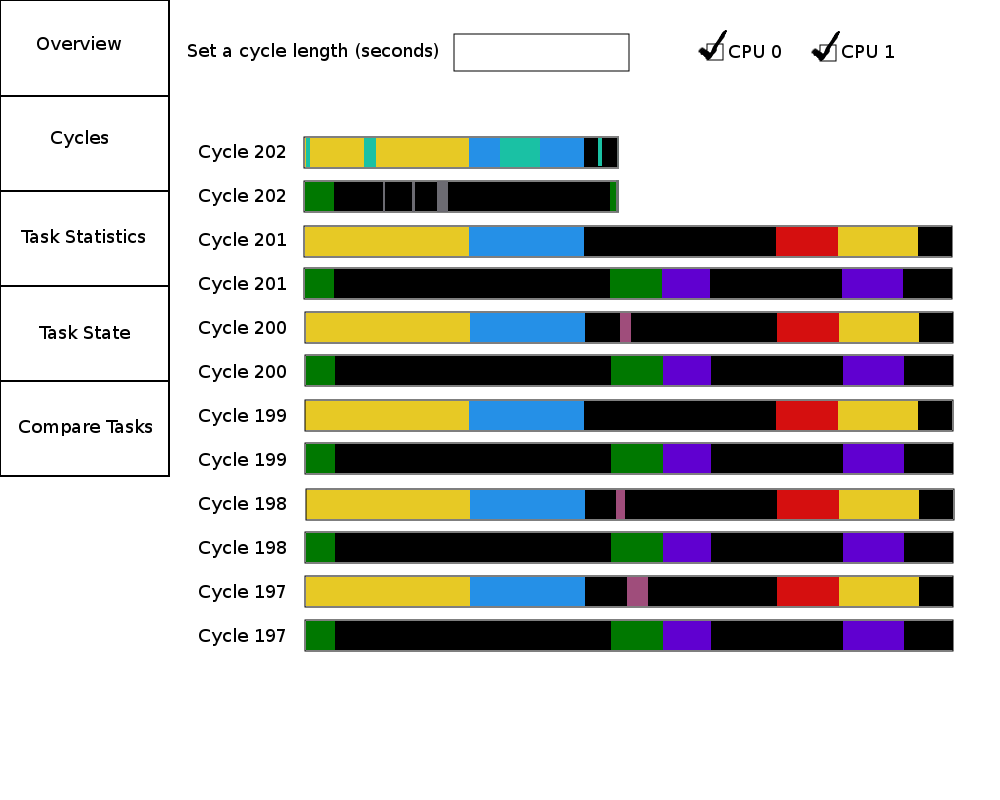
\includegraphics[width=4in]{futureCycles.png}
\caption{A mockup of how we envision the new Cycles page could look with
interleaved graphs.}
\end{center}
\end{figure}

It is also possible that the loaded files will contain more than two CPU's.
For clear visual purposes, we only want to be displaying two CPU's graphs
on the Cycles page. In the case that we have more than two CPU's, 
we would hope to be able to paginate the graphs. 

\section{Speed} %Wendy
The data SpaceX will be using with our tool is very large, and becomes even
larger once we have parsed it. As a result, some parts of the tool load slowly. One main fix we have
implemented is batch loading the list of events on the main page so that the
user can start interacting with the tool without waiting to load the entire
table, especially since all of the table is typically not needed.

Having done some profiling, we know that pulling data from IndexedDB is the
slowest part of our application, but at this point in time we do not have a way
to fix this.

\section{Scalability}
Typically for trace files using more than 4
cores, the parsed version will be too large for IndexedDB to load, and
sometimes too large for the parser to handle as well.

There are two possibilities for fixing this. One is to prune the JSON or
find a more compressed method of storing the data. The other is to find a
substitute for IndexedDB that can store more data.

\chapter{Appendices}
\newpage
\appendix
\renewcommand{\thesection}{\Alph{section}}
\section{Example JSON} \label{App:AppendixA}

\begin{verbatim}
Tasks
{
  [name: python, pid: 34602, events: [1,5,8,23,52...], 
   preemptedBy: [kworker, systemhousekeeper,...], 
   preemptionCount: 564, totalRuntime: 10000,
   totalWaittime: 20386, totalSleeptime: 52], [name:...],

   ...   
}

Events
{
  [name: python, 
   pid: 34602, 
   cpu: 2, startTime: 12500, 
   eventType: sched_switch,
   extraInfo: prev_comm=trace-cmd prev_pid=34602 
       prev prio = 120 prev_state=S ==> next_comm=swapper/2 
       next_pid=300 next_prio=120 kworker-2418 [001]
       1681.955177, 
   activeName: kworker, 
   activePID=300], 
   [name:...], 

   ...
}
\end{verbatim}
\newpage

\newpage
\section{Glossary}
\begin{itemize}[ ]
\item {\bf Blocked:} When a task is runnable but another task is running on the same CPU, thereby blocking it from being able to run.
\item {\bf Cycle:} The interval between the regular deadlines that tasks running on a SpaceX rocket need to meet.
\item {\bf CPU:} The Central Processing Unit; the part of the computer that carries out instructions.
\item{\bf Event:} A specific activity of a task taking place at a single point in time that can denote a change in its state or some other action.
\item {\bf PID:} A process identifier; a number attatched to a process that is unique to that process.
\item {\bf Preemption:} When a running task is blocked by another program starting to run on the same CPU. 
\item {\bf Priority Inversion:} When a high-priority task is indirectly blocked by something of
lower priority using a shared resource that the higher priority task needs in
order to run. 
\item{\bf Process:} A program that can have many threads.
\item {\bf Running:} The state of a task when it is being executed on the CPU.
\item {\bf Task:} A single thread of a process; a series of events.
\item {\bf Waiting:} The state of a task when it cannot run, due to being blocked or waiting on some piece of information.
\end{itemize}

\newpage
\section{How to Package the Application}
If changes have been made to any files within a cloned copy of the repository,
the application can be repackaged with these steps.

\begin{enumerate}
  \item Navigate into the top level of the directory, which contains
    \texttt{package.json}
  \item Move the spaceshark script, README, and parser jar files to the parent directory
    and delete the rest of the parser files
  \item run
    \begin{center}\texttt{zip -r ../\${PWD\#\#*/}.nw *}\end{center} here, which will create a file
    called \texttt{SpaceX14.nw} in the parent directory
  \item Download a copy of node-webkit from
    \texttt{https://github.com/nwjs/nw.js} and
    place it in the directory above the Spaceshark repository
  \item Move to this directory and run 
    \begin{center}\texttt{cat nw SpaceX14.nw >
      app \&\& chmod +x app}\end{center}
  \item Zip together the app file, \texttt{nw.pak}, \texttt{icudtl.dat}, the spaceshark script,
    README, and parser jar files
\end{enumerate}

\newpage
\section{Debugging}
To display a web console for debugging, within \texttt{package.json} change the line
\texttt{toolbar: false} to \texttt{toolbar: true}. A gear icon should now appear in the
top right corner of the application when it is launched. When clicked, this
displays a web console that allows the user to view current css properties,
set breakpoints in code, and view the resources within IndexedDb and local
storage.
\end{document}
